\chapter{DENEYSEL DOĞRULAMA}
\label{chap:deney}

Bölüm~\ref{chap:anahtarlama} ve Bölüm~\ref{chap:sin3} içinde benzetim düzeyinde incelenen klasik anahtarlama, nötr anahtar susturma ve susturma+Sin\textsuperscript{3} yöntemleri, geliştirilen üç fazlı T-tipi prototipin tek faz kolunda, düşük güç koşulunda karşılaştırılmıştır. Bölümde deney düzeneği, güç donanımı, denetim ve ölçüm zinciri testleri yeniden üretecek ayrıntıda tanıtılmakta; mevcut deney kayıtları kanıt sınırlarıyla birlikte değerlendirilmekte ve benzetim modelinin deney özetine kalibrasyonu (Kesim~\ref{sec:kalibrasyon}) verilmektedir. Tez kapsamında yeni deney yapılmamıştır; kayıtlar mevcut arşivden alınmış, metin, tablo ve ekran değerleri kaynak içi tutarlılık bakımından denetlenmiştir.

\textbf{Deneysel kanıtın kapsamı.} Eldeki deneysel kanıt üç yönteme ait PC yazılımı ekranları, osiloskop ekranları ve her yöntem için tek satırlık bir deney özet tablosudur (Tablo~\ref{tab:gelen-excel-senaryolar}). Enerjilendirme sırası, başlangıç koşulları, kararlı duruma geçiş ölçütü ve ölçüm süresini içeren deney protokolü; ham PC/Modbus ve osiloskop kayıtları; tekrar sayısı ve analizör kalibrasyon belgeleri belgelenmemiştir. Deney sonuçları, ekran ve özet tablosu düzeyinde destekleyici kanıt olarak kullanılmaktadır. Ölçüm belirsizliği yalnız üretici toleransları ve okuma çözünürlüğünden kestirilebilmekte, istatistiksel yayılım hesaplanamamaktadır. Benzetim modeli deney özetinin etkin ve reaktif gücüne kalibre edilmiş, diğer büyüklükler bağımsız karşılaştırma olarak raporlanmıştır (Kesim~\ref{sec:kalibrasyon}). Protokol ve ham kayıt eksikliği Bölüm~\ref{chap:sonuc} içinde sınırlılık olarak yer almaktadır.

\section{Deney Düzeneği ve Güç Donanımı}

Deney düzeneği, yaklaşık 20--25~kW güç dönüştürme kapasitesi hedeflenerek düşey bir pano üzerine bakır baralarla modüler biçimde kurulmuştur. Akım sensörü boyutlandırma hesabında prototip gücü \SI{20}{\kilo\volt\ampere} olarak verilmiştir; güç birimi ve anma değeri arasındaki fark, prototip etiketi veya tasarım dosyası bulunmadan tek bir anma değerinde birleştirilmemiştir. Raporlanan deneylerin yaklaşık \SI{2.3}{\ampere} faz akımında gerçekleştirilmesi, mevcut sonuçların anma gücü değil düşük güç doğrulaması olduğunu göstermektedir.

Şekil~\ref{fig:deney-duzenegi-genel}; varyak modülü, evirici panosu, bilgisayar ve osiloskopları aynı görünümde vermektedir. Varyak modülünde enerji bağlantıları, şalt ve koruma ekipmanları, akım transformatörleri ve AA enerji analizörü bulunmakta; üç faz bağımsız varyaklarla ayarlanabilmektedir. Aşırı akım, kaçak akım, topraklama ve acil durdurma önlemleri mevcuttur; eşik ve açma süreleri kaynak kayıtlarda yer almamaktadır.

\begin{figure}[htbp]
  \centering
  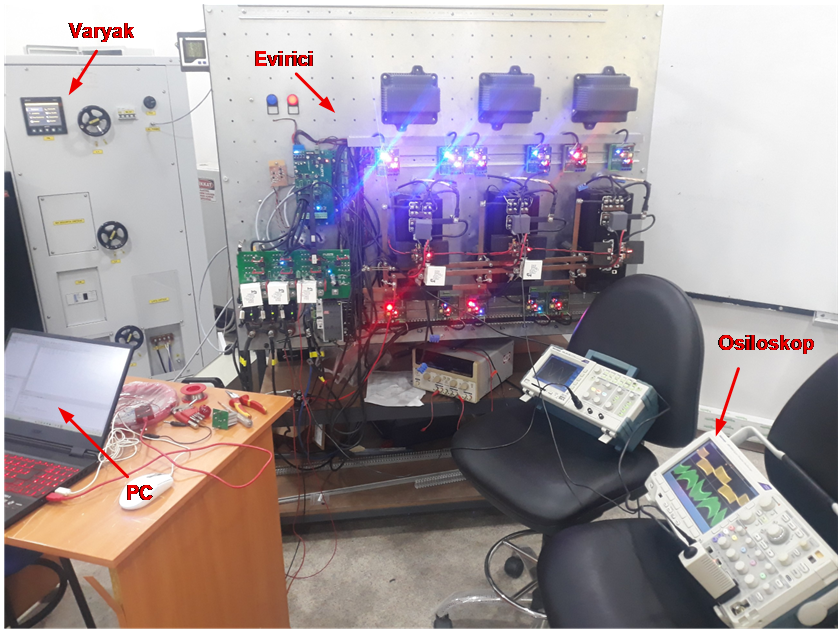
\includegraphics[width=0.95\textwidth]{deneysel/onceki_tez_sekil_5_1_deney_duzenegi.png}
  \caption{Deney ve ölçme düzeneklerinin genel görünümü.}
  \label{fig:deney-duzenegi-genel}
\end{figure}

Şekil~\ref{fig:deney-evirici-genel}, evirici donanımının önden genel görünümünü sunmaktadır. Üç faza ait güç modülleri, kontrol ve ölçüm kartları, DA bara bağlantıları ve yardımcı beslemeler aynı pano üzerindedir; genel görünüm, numaralı ayrıntıların verildiği Şekil~\ref{fig:deney-donanim-kartlar} için yerleşim bağlamı sağlamaktadır.

\begin{figure}[htbp]
  \centering
  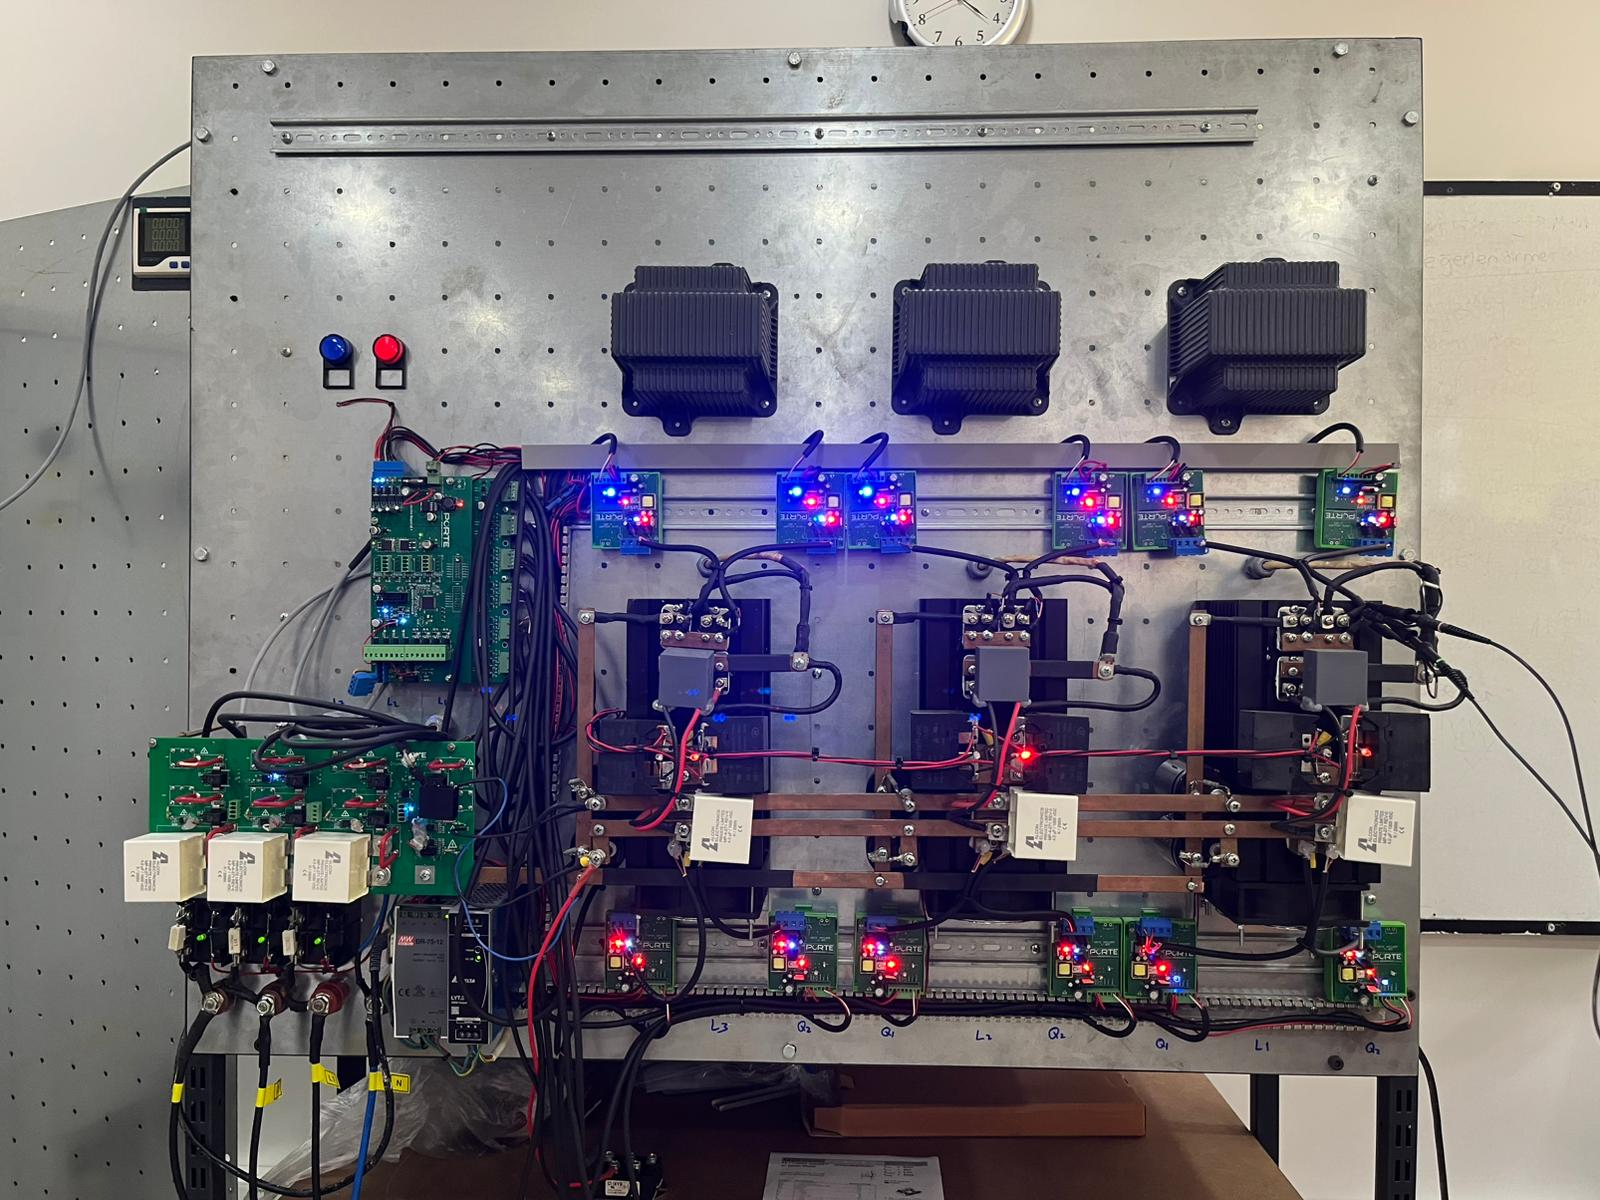
\includegraphics[width=0.88\textwidth]{deneysel/onceki_tez_sekil_5_2_evirici_donanimi.jpeg}
  \caption{Evirici donanımının genel görünümü.}
  \label{fig:deney-evirici-genel}
\end{figure}

Şekil~\ref{fig:deney-donanim-kartlar} üzerindeki 1--14 numaraları doğrudan Tablo~\ref{tab:deney-alt-birimler} içindeki açıklamalara karşılık gelmektedir.

\begin{figure}[htbp]
  \centering
  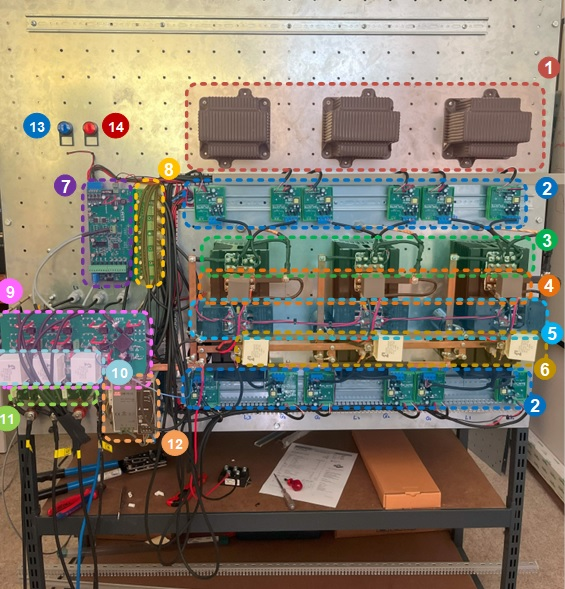
\includegraphics[width=0.72\textwidth]{deneysel/onceki_tez_sekil_5_3_donanim_alt_birimleri.jpeg}
  \caption{Evirici donanımı ve alt birimlerinin numaralı tanıtımı.}
  \label{fig:deney-donanim-kartlar}
\end{figure}

\clearpage
\begin{table}[htbp]
  \centering
  \caption{Evirici donanımının alt birimleri.}
  \label{tab:deney-alt-birimler}
  \small
  \begin{tabularx}{0.94\textwidth}{X X}
    \toprule
    1. LCL filtrelerin $L_1$ bobinleri & 2. IGBT kapı sürme kartları \\
    3. Nötr IGBT'leri & 4. Yükseltici (boost) diyotları \\
    5. Fonksiyon değiştirme röleleri & 6. Snubber kapasitörleri \\
    7. Kontrol kartı & 8. Tampon (buffer) kartı \\
    9. Ölçme kartı & 10. LCL filtre kapasitörleri \\
    11. Ani akım (inrush) röleleri & 12. Kumanda beslemeleri \\
    13. Şarj fonksiyonu lambası & 14. Deşarj fonksiyonu lambası \\
    \bottomrule
  \end{tabularx}
\end{table}

Şekil~\ref{fig:deney-faz-donanim-1} ve Şekil~\ref{fig:deney-faz-donanim-2}, aynı faz kolunun iki farklı açıdan çekilmiş ayrıntılarını göstermektedir; her iki görseldeki 1--8 numaraları Tablo~\ref{tab:deney-faz-komponentler} ile birlikte okunmalıdır. İki görüntünün ayrı tutulması; boost diyotları, fonksiyon değiştirme röleleri, DA bara ve snubber kapasitörleri, soğutma düzeni, sürücü kartı ve $L_1$ bobininin fiziksel konumunu kaybetmeden izlemeyi sağlamaktadır.

\begin{figure}[htbp]
  \centering
  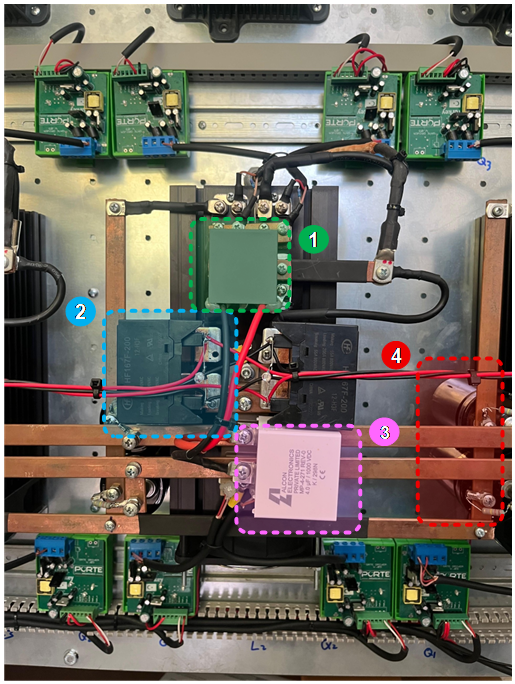
\includegraphics[height=0.68\textheight]{deneysel/onceki_tez_sekil_5_4_faz_donanimlari_1.png}
  \caption{Eviricinin bir fazına ait donanımlar, birinci görünüm.}
  \label{fig:deney-faz-donanim-1}
\end{figure}

\begin{figure}[htbp]
  \centering
  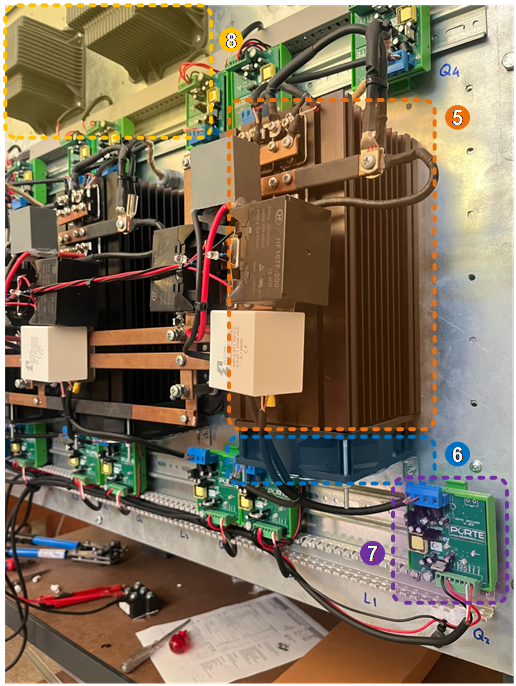
\includegraphics[height=0.68\textheight]{deneysel/onceki_tez_sekil_5_5_faz_donanimlari_2.png}
  \caption{Eviricinin bir fazına ait donanımlar, ikinci görünüm.}
  \label{fig:deney-faz-donanim-2}
\end{figure}

\clearpage
\begin{table}[htbp]
  \centering
  \caption{Şekil~\ref{fig:deney-faz-donanim-1} ve Şekil~\ref{fig:deney-faz-donanim-2}'deki faz donanımı bileşenleri.}
  \label{tab:deney-faz-komponentler}
  \small
  \begin{tabularx}{0.94\textwidth}{X X}
    \toprule
    1. Boost diyotları ve kondansatörü & 2. Fonksiyon değiştirme röleleri \\
    3. Snubber kondansatörleri & 4. DA bara elektrolitik kondansatörleri \\
    5. IGBT soğutucu & 6. Yüksek devirli soğutma fanı \\
    7. IGBT kapı sürme kartı & 8. LCL filtre $L_1$ bobini \\
    \bottomrule
  \end{tabularx}
\end{table}

Şekil~\ref{fig:deney-giris-devresi}, evirici giriş devresini ve 1--6 ile işaretlenmiş yardımcı donanımları göstermektedir; numaraların karşılığı Tablo~\ref{tab:deney-giris-komponentler} içindedir. Giriş bölümünün ayrı verilmesi; inrush röleleri, sigorta, yardımcı kaynaklar, EMI filtresi, kontrol kartı ve tampon kartının güç katıyla bağlantısını görünür kılmaktadır.

\begin{figure}[htbp]
  \centering
  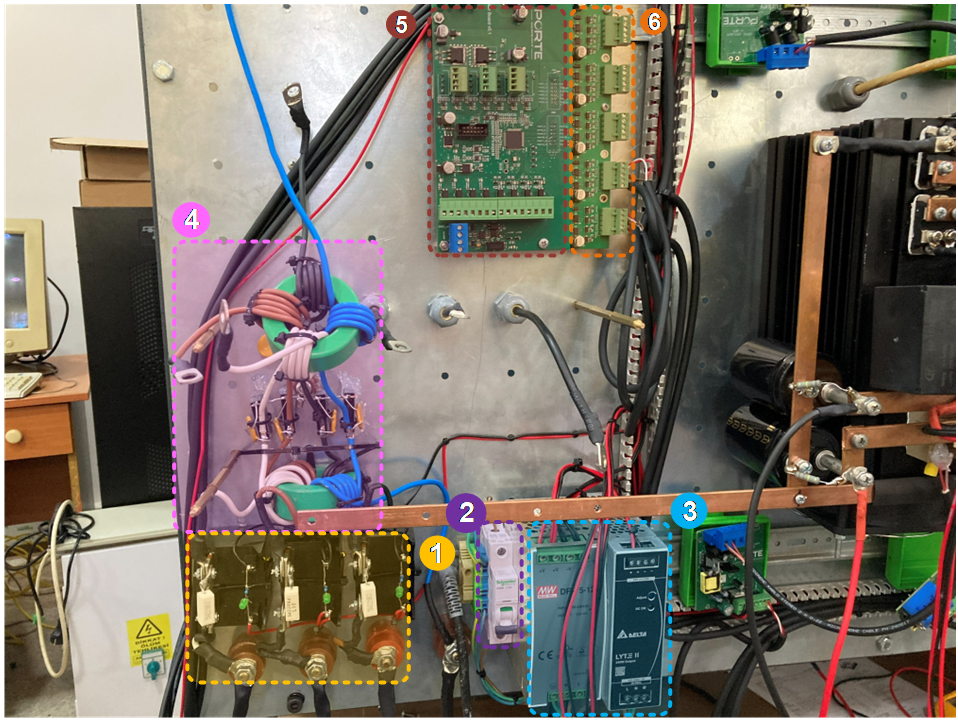
\includegraphics[width=0.94\textwidth]{deneysel/onceki_tez_sekil_5_6_giris_devresi.png}
  \caption{Evirici giriş devresinin ayrıntı görünümü.}
  \label{fig:deney-giris-devresi}
\end{figure}

\clearpage
\begin{table}[htbp]
  \centering
  \caption{Evirici giriş kısmına ait bileşenler.}
  \label{tab:deney-giris-komponentler}
  \small
  \begin{tabularx}{0.94\textwidth}{X X}
    \toprule
    1. Ani akım (inrush) röleleri & 2. Evirici açma kapama sigortası \\
    3. 12 V--24 V güç kaynakları & 4. EMI filtre \\
    5. Kontrol kartı & 6. Tampon (buffer) kartı \\
    \bottomrule
  \end{tabularx}
\end{table}

\section{Kontrol Kartı, Tampon Kartı ve Kapı Sürücüsü}

Şekil~\ref{fig:deney-kontrol-buffer}, kontrol ve tampon kartlarını numaralı işlevleriyle göstermektedir. Kontrol kartında RS485 haberleşme birimi, optoizole giriş/çıkışlar, DA bara ve akım ölçüm dönüştürme devreleri, PIC32MK ailesi mikrodenetleyici, lineer regülatörler ve röle/fan çıkış katları bulunmaktadır. Tampon kartı, mikrodenetleyicinin \SI{3.3}{\volt} tek uçlu (single-ended) PWM işaretlerini diferansiyel sinyal çiftlerine dönüştürmek ve uzun ekranlı kablolarda ortak-mod gürültü etkisini azaltmak amacıyla kullanılmıştır. Fotoğraftaki numaralar sırasıyla şu işlevleri gösterir: (1) RS485 haberleşme; (2)--(3) optoizole giriş ve çıkışlar; (4) diferansiyel DA bara gerilimini tek uçlu biçime dönüştüren ölçüm katı; (5) ölçüm, haberleşme ve kontrol algoritmalarını yürüten PIC32MK mikrodenetleyici; (6) akım ölçüm dönüştürme katı; (7) \SI{5}{\volt} lineer regülatörler; (8) röle ve fanlar için MOSFET güç çıkışları; (9) \SI{9}{\volt} anahtarlamalı regülatör; (10) PWM tampon kartının \SI{9}{\volt} beslemesi; (11) tek uçlu PWM işaretlerini diferansiyel çiftlere dönüştüren kat.

\begin{figure}[htbp]
  \centering
  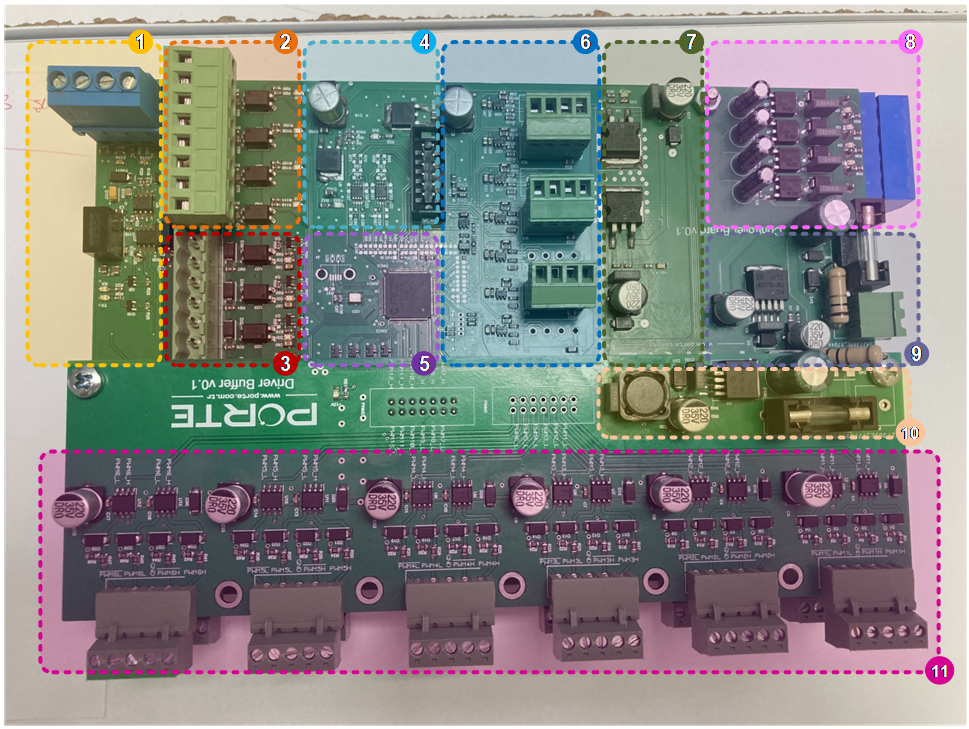
\includegraphics[width=0.90\textwidth]{deneysel/onceki_tez_sekil_5_7_kontrol_buffer.png}
  \caption{Kontrol kartı ve tampon kartının numaralı görünümü.}
  \label{fig:deney-kontrol-buffer}
\end{figure}

PWM1--PWM6 kanallarının yüksek ve alçak işaretleri tampon kartında diferansiyel çiftlere dönüştürülmekte; yaklaşık \SI{12}{\volt} genlikte, tek yönlü iletim amacıyla H-köprü tabanlı bir sürme çözümü kullanılmaktadır. Gerçek PWM kaynak kodu, ölü zaman, minimum darbe süresi ve çıkış gecikmeleri mevcut olmadığından zincirin zamanlama performansı henüz doğrulanamamıştır.

Şekil~\ref{fig:deney-igbt-surucu}, ADuM4135 tabanlı IGBT kapı sürme kartını göstermektedir. Diferansiyel giriş, desatürasyon koruması, aktif Miller kenetleme ve düşük gerilim kilitleme özellikleri sürücü seçiminin gerekçeleridir: diferansiyel giriş uzun PWM hatlarındaki ortak-mod gürültüsüne bağışıklık sağlar; desatürasyon koruması aşırı akımda IGBT komutunu donanımsal olarak keser; aktif Miller kenetleme yüksek frekanslı anahtarlamada hatalı iletime geçme (false turn-on) riskini azaltır. Bütün sürücülerden gelen FAULT çıkışları kontrol kartında toplanmakta ve ortak RESET işareti sürücülere paralel dağıtılmaktadır; böylece donanım koruması ile denetim yazılımı arasında bir hata yönetim zinciri oluşmaktadır.

\begin{figure}[htbp]
  \centering
  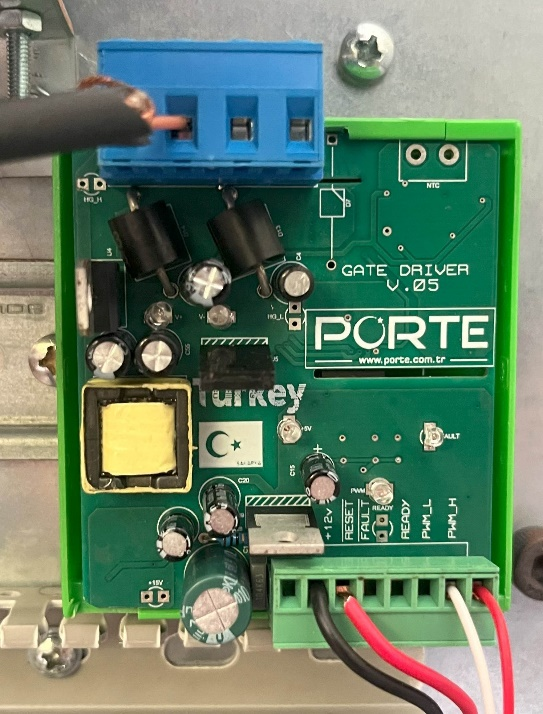
\includegraphics[height=0.64\textheight]{deneysel/onceki_tez_sekil_5_8_igbt_surucu.jpeg}
  \caption{IGBT kapı sürme devresi.}
  \label{fig:deney-igbt-surucu}
\end{figure}

\clearpage
\section{Gerilim ve Akım Ölçme Devreleri}

Faz--nötr gerilimleri ile pozitif ve negatif DA bara gerilimleri, AMC1200 tabanlı izole ölçüm devreleriyle alınmaktadır; ölçüm kartının ofset, ADC aralığı ve DA bara ölçüm aralığı Tablo~\ref{tab:sistem-parametreleri} içindedir. AMC1200'ün gerilim kazancı 8 olduğundan girişte izin verilen en yüksek genlik \SI{162.5}{\milli\volt} olarak hesaplanmış; faz ve DA bara ölçümleri için ayrı gerilim bölücüler kullanılmıştır. Faz ölçüm sınırı anlık yaklaşık \SI{387}{\volt}'tur.

Mikrodenetleyicideki yedi ADC kanalının üçü faz--nötr gerilimlerine, ikisi pozitif ve negatif DA bara gerilimlerine ayrılmıştır. Faz ölçümleri AMC1200 çıkışlarından ekranlı kabloyla diferansiyel olarak taşınmış ve RC örtüşme önleme (anti-aliasing) filtrelerinden geçirilmiştir. DA bara kanallarında diferansiyel işaretler enstrümantasyon yükselteciyle işlenip \SI{1.3}{\volt} ofset eklenerek tek uçlu biçime dönüştürülmektedir. 12 bit ADC gösterimi, diferansiyel sayısal aralığı yaklaşık $-2047$ ile $+2048$ arasında tanımlamaktadır.

Dört telli T-tipi yapıda nötr noktasının kayması iki DA bara kondansatörünün gerilimlerini eşitsizleştirebileceğinden pozitif ve negatif bara kanalları sürekli izlenmekte; eşik aşımında mikrodenetleyici FAULT üretip PWM çıkışlarını kesmektedir. AMC1200 giriş beslemesi RFM-0505S izole dönüştürücü ile sağlanmış; dönüştürücü çıkışındaki regülasyon zayıflığını azaltmak için TCR2EF250 düşük gerilim düşümlü regülatör kullanılmıştır. Ölçüm zinciri böylece yalnız ölçekleme değil, izolasyon ve nötr nokta koruması görevlerini de üstlenmektedir.

Akım ölçümünde HLSR 20-P/SP33 Hall etkili sensör kullanılmıştır. Sensör kazancı ve ölçülebilir simetrik tepe akımı Tablo~\ref{tab:sistem-parametreleri} içindedir; tepe sınırın RMS karşılığı yaklaşık \SI{39.9}{\ampere}'dir. Faz başına akım tasarım değeri ve yüzde 20 paylı üst sınırı aynı tabloda verilmiştir. Hesaplar nominal direnç değerlerine dayanır; gerçek direnç toleransları, ADC kalibrasyonu ve sensör sıcaklık sapmasıyla doğrulanmamıştır.

Ani faz ve kondansatör akımlarının sınırlandırılması amacıyla kullanılan pencere karşılaştırıcı devre Şekil~\ref{fig:deney-pencere-karsilastirici} üzerinde verilmiştir. Devrede üst eşik \SI{2.0}{\volt}, alt eşik \SI{0.6}{\volt} olarak, sensör referansına simetrik ayarlanmıştır. Eşiklerin referanstan uzaklığı, sensör kazancıyla Tablo~\ref{tab:sistem-parametreleri} içindeki aşırı akım eşiğine karşılık gelmektedir. Eşik dışına çıkıldığında FAULT işareti kontrol kartında harici kesme oluşturarak PWM çıkışlarını kesmektedir.

\begin{figure}[htbp]
  \centering
  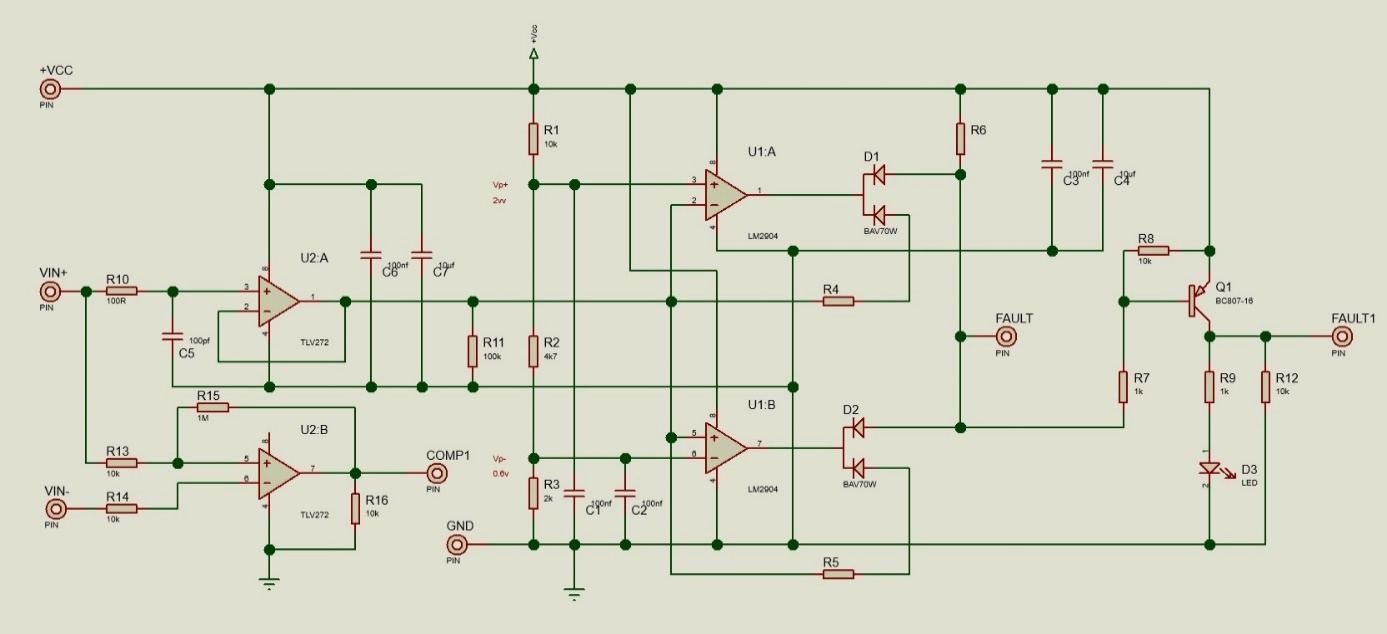
\includegraphics[width=0.96\textwidth]{deneysel/onceki_tez_sekil_5_9_pencere_karsilastirici.jpeg}
  \caption{Pencere karşılaştırıcı devresi.}
  \label{fig:deney-pencere-karsilastirici}
\end{figure}

Şekil~\ref{fig:deney-pencere-dalga}, harici bir deneme kartının DAC çıkışıyla uygulanan giriş işareti ve pencere karşılaştırıcının FAULT çıkışını göstermektedir. İmleç seviyeleri \SI{2.0}{\volt} ve \SI{0.6}{\volt} olarak ayarlanmış; giriş sınırların dışına çıktığında ikinci kanal işaretinin lojik sıfıra indiği gözlenmiştir. Kayıt, koruma mantığının işlevsel örneğidir; gecikme süresi ve gerçek kısa devre kesme enerjisi aynı görüntüden çıkarılamaz.

\begin{figure}[htbp]
  \centering
  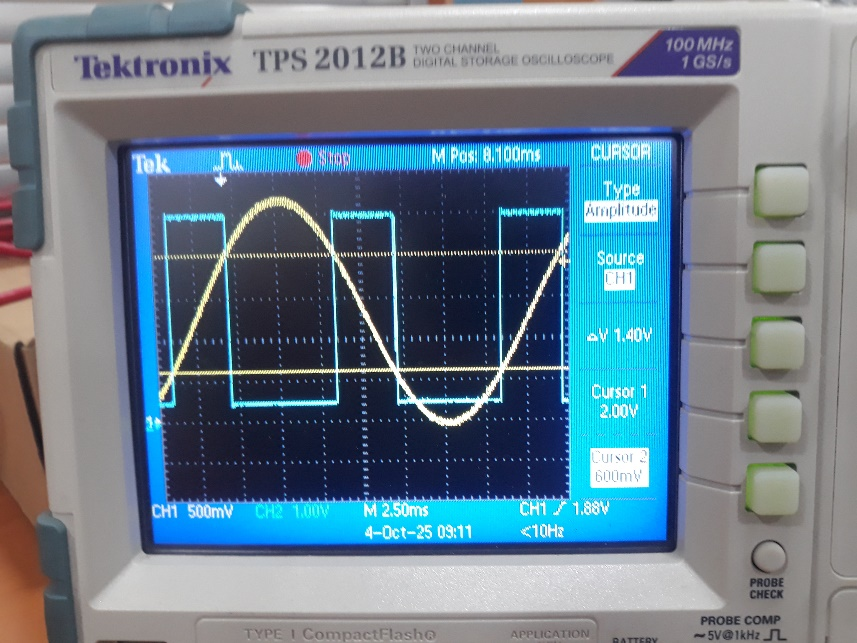
\includegraphics[width=0.88\textwidth]{deneysel/onceki_tez_sekil_5_10_pencere_dalga.jpeg}
  \caption{Pencere karşılaştırıcı giriş ve çıkış gerilim dalga şekilleri.}
  \label{fig:deney-pencere-dalga}
\end{figure}

Şekil~\ref{fig:deney-olcum-karti}; HLSR akım sensörleri, AMC1200 izole ölçüm kanalları ve akım probu bağlantı iletkenlerini içeren ölçüm kartını göstermektedir. Kart üzerindeki \SI{4}{\milli\metre\squared} kesitli ters-U biçimli iletkenler; faz başına $L_1$ akımı, kondansatör akımı ve faz akımının ayrı ayrı osiloskop probuyla ölçülmesini sağlamaktadır. TLV431 referansları ve MC33269 regülatörleri ölçüm beslemesi ile \SI{1.3}{\volt} ofset üretiminde kullanılmıştır.

\begin{figure}[htbp]
  \centering
  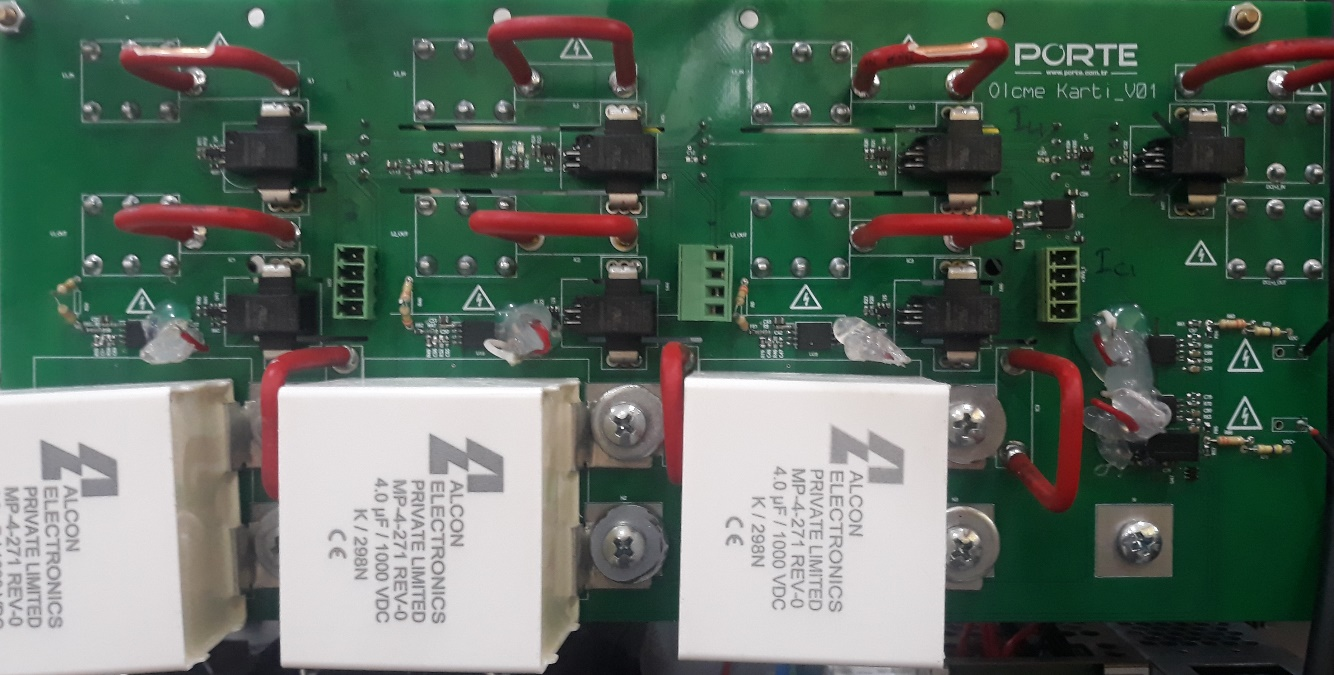
\includegraphics[width=0.96\textwidth]{deneysel/onceki_tez_sekil_5_11_olcum_karti.jpeg}
  \caption{Ölçüm kartı.}
  \label{fig:deney-olcum-karti}
\end{figure}

\section{DA ve AA Güç Analizörleri}

DA bara gerilimi, akımı ve gücü Accuenergy AcuDC240 analizörüyle ölçülmüştür; üretici akım ve gerilim için yüzde 0,2, güç ve enerji için yüzde 0,5 hata toleransı bildirmektedir. Şekil~\ref{fig:deney-acudc240}(a) cihazın pano üzerindeki konumunu, Şekil~\ref{fig:deney-acudc240}(b) üretici dokümanındaki şönt bağlantısını göstermektedir.

\begin{figure}[htbp]
  \centering
  \begin{subfigure}[t]{0.46\textwidth}
    \centering
    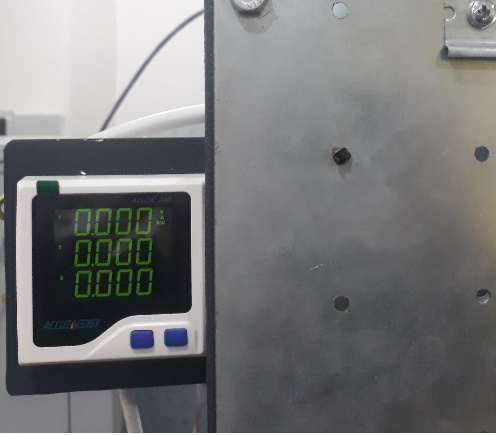
\includegraphics[width=\linewidth]{deneysel/onceki_tez_sekil_5_12a_acudc240.jpeg}
    \caption{Evirici donanımı üzerindeki AcuDC240.}
  \end{subfigure}\hfill
  \begin{subfigure}[t]{0.50\textwidth}
    \centering
    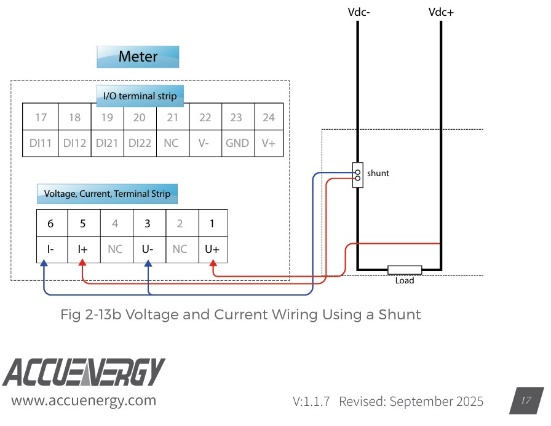
\includegraphics[width=\linewidth]{deneysel/onceki_tez_sekil_5_12b_acudc240_baglanti.jpeg}
    \caption{DA analizörü ve şönt bağlantı şekli.}
  \end{subfigure}
  \caption{AcuDC240 DA bara analizörü ve bağlantısı.}
  \label{fig:deney-acudc240}
\end{figure}

Prototipte şönt direnci DA baranın negatif terminaline bağlanarak alçak-taraf akım ölçümü yapılmıştır. Şekil~\ref{fig:deney-sont-baglanti}, \SI{20}{\ampere}/\SI{60}{\milli\volt} şönt direncin fiziksel bağlantısını göstermektedir. Şöntün ölçüm uçları koaksiyel ve ekranlı kabloyla analizöre taşınmış; DA gerilim girişinde yüksek izolasyon dayanımlı kablo kullanılmıştır.

\begin{figure}[htbp]
  \centering
  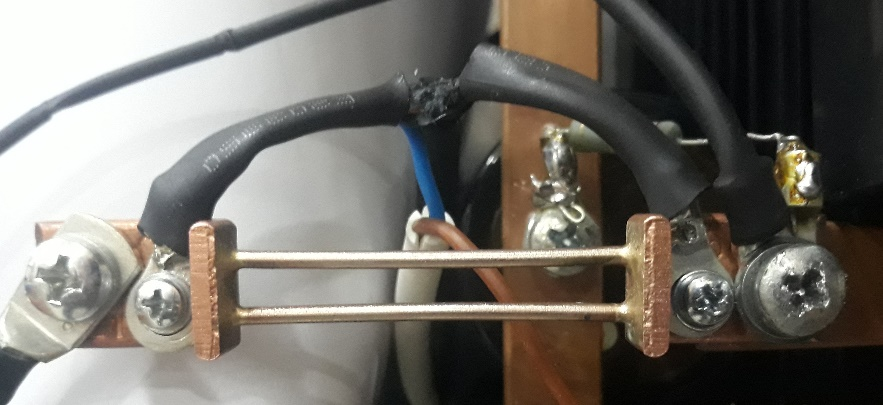
\includegraphics[width=0.94\textwidth]{deneysel/onceki_tez_sekil_5_13_sont_baglanti.jpeg}
  \caption{\SI{20}{\ampere}--\SI{60}{\milli\volt} şönt direnç bağlantısı.}
  \label{fig:deney-sont-baglanti}
\end{figure}

AA tarafta Entes EMK-01 analizörü ve 50/5 oranlı, \SI{5}{\volt\ampere}, Class~0.1 akım transformatörleri kullanılmıştır. Üç faz ve nötr hattı için dört akım transformatörü bağlanmış; faz--nötr gerilimleri, faz/nötr akımları, aktif ve reaktif güç ile toplam THD değerleri Modbus RTU üzerinden okunmuştur. Şekil~\ref{fig:deney-emk01}(a) analizörü, Şekil~\ref{fig:deney-emk01}(b) üreticinin bağlantı düzenini vermektedir.

\begin{figure}[htbp]
  \centering
  \begin{subfigure}[t]{0.43\textwidth}
    \centering
    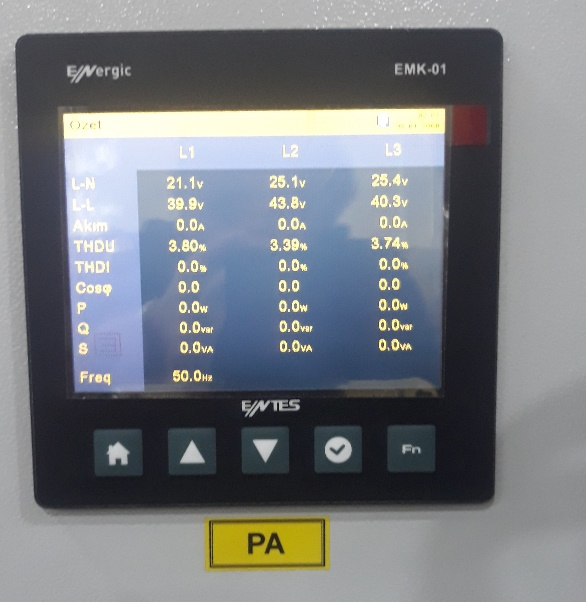
\includegraphics[width=\linewidth]{deneysel/onceki_tez_sekil_5_14a_emk01.jpeg}
    \caption{EMK-01 AA analizörü.}
  \end{subfigure}\hfill
  \begin{subfigure}[t]{0.53\textwidth}
    \centering
    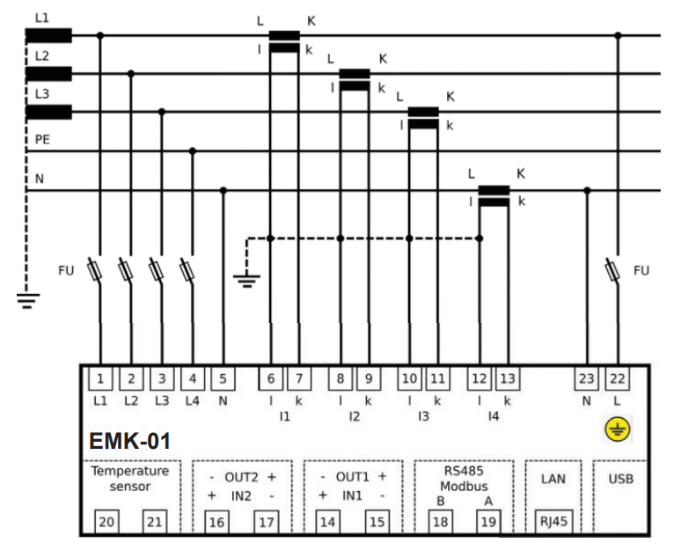
\includegraphics[width=\linewidth]{deneysel/onceki_tez_sekil_5_14b_emk01_baglanti.png}
    \caption{Üretici tarafından önerilen bağlantı şekli.}
  \end{subfigure}
  \caption{EMK-01 AA analizörü ve bağlantısı.}
  \label{fig:deney-emk01}
\end{figure}

\section{PC Ana Kumanda Yazılımı ve Veri Toplama}

PC ana kumanda yazılımı; EMK-01, AcuDC240 ve kontrol kartından RS485/Modbus RTU üzerinden veri almak, anlık değerleri grafikleştirmek ve verim hesabına temel oluşturmak amacıyla geliştirilmiştir. Şekil~\ref{fig:deney-pc-arayuzu} yazılımın arayüzünü göstermektedir. Bir veri çevrimi yaklaşık \SI{1}{\second} sürmekte; önce DA analizörü, en fazla yaklaşık \SI{50}{\milli\second} sonra AA analizörü okunmaktadır. Yapı kararlı durum eğilimleri için kullanılabilir; hızlı geçici rejimlerin tam eşzamanlı karşılaştırılması için yeterli değildir.

Haberleşme hızı cihazların izin verdiği en yüksek değer olan 38400 baud seçilmiş; veri sırası DA analizörü, AA analizörü ve kontrol kartı biçiminde kurulmuştur. Yazılımın karşılaştırma seti verim, THD, güç faktörü, faz akımı, faz--nötr gerilimi ve DA bara geriliminden oluşmaktadır. Osiloskop kanal adlarında ``kontrolör çıkışı'' ifadesi geçmektedir. Senaryo tanımlarında S1--S3 açık çevrim modülasyonla çalışır ve akım geri beslemesi yalnız S4'te bulunur (Kesim~\ref{sec:s4-kapali-cevrim}); kanal adındaki ifade, modülasyon komutu olarak okunmuştur. Donanım yazılımı belgelenmediğinden okuma, benzetim modelinin yapısına dayanmaktadır.

\begin{figure}[htbp]
  \centering
  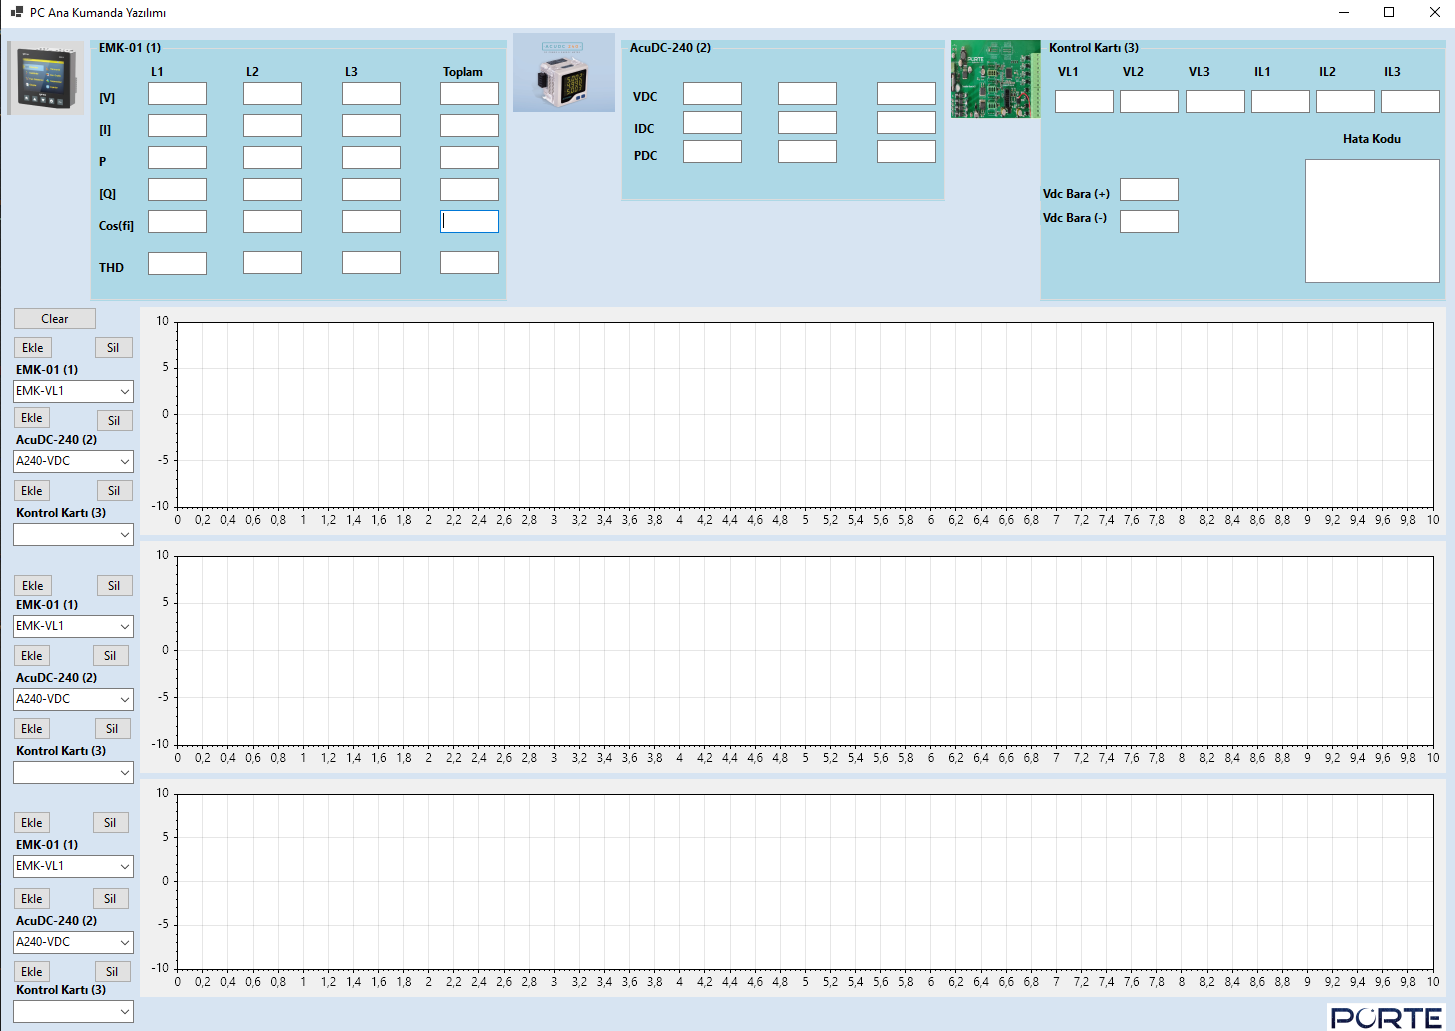
\includegraphics[width=0.98\textwidth]{deneysel/onceki_tez_sekil_5_15_pc_arayuzu.png}
  \caption{Haberleşme sistemi arayüzü.}
  \label{fig:deney-pc-arayuzu}
\end{figure}

Ortak hedef çalışma koşulu; DA bara gerilimi yaklaşık \SI{400}{\volt}, faz--nötr gerilimi yaklaşık \SI{130}{\volt}, faz akımı yaklaşık \SI{2.3}{\ampere} ve birim güç faktörüne yakın işletim olarak tanımlanmıştır. Gerçek ekran ve metin kayıtları yöntemler arasında farklı DA bara ve faz gerilimleri bulunduğunu göstermektedir. Verim, THD ve ters akım ölçütleri Eşitlik~\eqref{eq:verim-tanimi}, Eşitlik~\eqref{eq:thd-rmse-tanimlari} ve Eşitlik~\eqref{eq:ters-akim-anahtarlama-olcutleri} ile ilişkilendirilmiştir.

\section{Klasik Anahtarlama Modu Deney Kayıtları}

Klasik yöntemde bütün anahtarlar tamamlayıcı sürülmekte ve düşük akımda senkron-buck benzeri ters akım yolu açık kalmaktadır. Deney özeti yüzde 92,5 verim, yüzde 15 akım THD'si, yaklaşık \SI{2.3}{\ampere} faz akımı, \SI{120}{\volt} faz--nötr gerilimi ve \SI{430}{\volt} DA bara gerilimi bildirmektedir.

Şekil~\ref{fig:deney-klasik-pc}, PC yazılımında klasik anahtarlama sırasında elde edilen grafiklerin tamamını göstermektedir; AA/DA analizör değerleri ile güç ve THD eğilimleri aynı arayüzde izlenmektedir.

\begin{figure}[htbp]
  \centering
  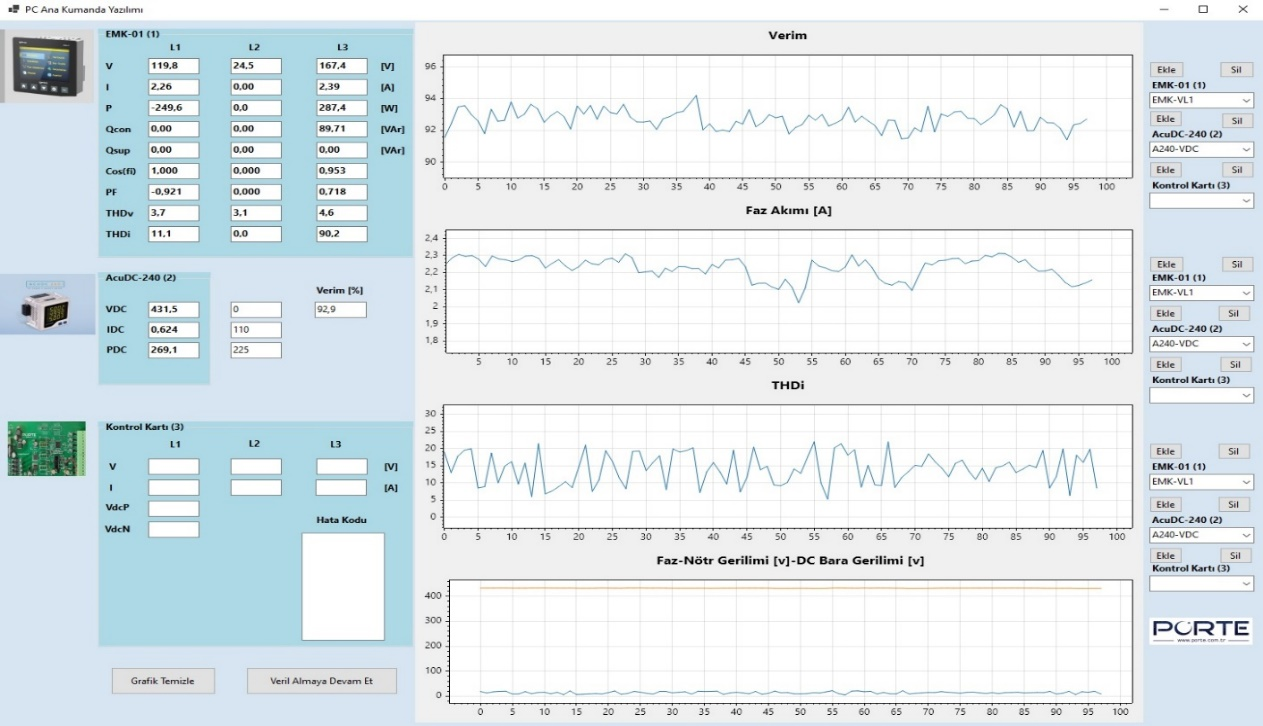
\includegraphics[width=0.98\textwidth]{deneysel/onceki_tez_sekil_5_16_klasik_pc.jpeg}
  \caption{Klasik anahtarlama sırasında PC yazılımında alınan grafikler.}
  \label{fig:deney-klasik-pc}
\end{figure}

Şekil~\ref{fig:deney-klasik-l1} üzerinde yukarıdan aşağıya kontrol işareti, şebeke gerilimi, işlemciden alınan ortalama endüktör akımı ve akım probuyla ölçülen $L_1$ akımı bulunmaktadır. Kayıt, anahtarlama dalgalanmasını ve akımın sıfır çevresindeki davranışını doğrudan göstermektedir.

\begin{figure}[htbp]
  \centering
  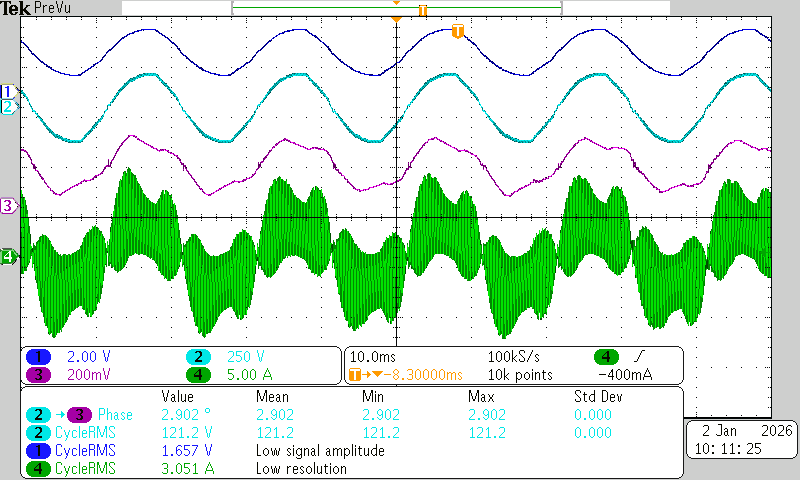
\includegraphics[width=0.94\textwidth]{deneysel/onceki_tez_sekil_5_17_klasik_l1.png}
  \caption{Klasik yöntemde kontrol işareti, şebeke gerilimi, ortalama endüktör akımı ve $L_1$ akımı.}
  \label{fig:deney-klasik-l1}
\end{figure}

Şekil~\ref{fig:deney-klasik-faz} üzerinde ilk üç kanal korunmuş, dördüncü kanalda faz akımı verilmiştir. $L_1$ akımı ile faz akımının ayrı kayıtlarda sunulması, filtre ve şebeke tarafındaki dalga biçimlerinin aynı fiziksel büyüklük olarak yorumlanmasını önlemektedir.

\begin{figure}[htbp]
  \centering
  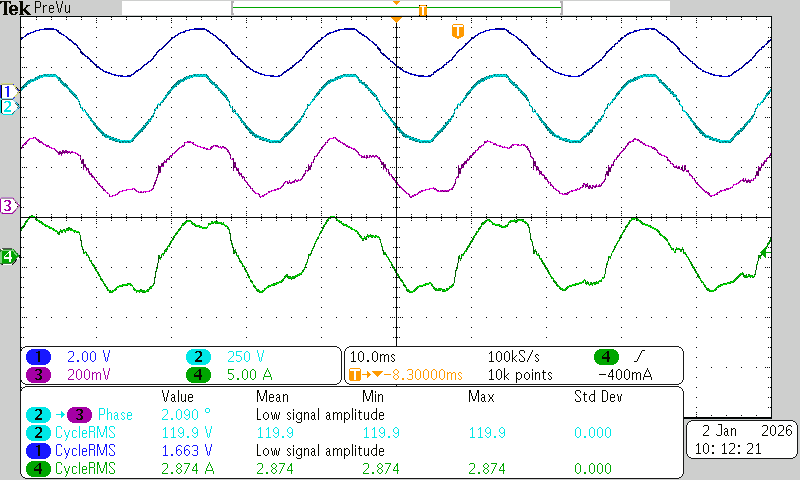
\includegraphics[width=0.94\textwidth]{deneysel/onceki_tez_sekil_5_18_klasik_faz.png}
  \caption{Klasik yöntemde kontrol işareti, şebeke gerilimi, ortalama endüktör akımı ve faz akımı.}
  \label{fig:deney-klasik-faz}
\end{figure}

\section{Nötr Anahtar Susturma Modu Deney Kayıtları}

Nötr anahtar susturma yönteminde ilgili yarım periyotta ters akım yolu kesilmekte, düşük görev oranında kesintili iletim ve üçüncü harmonik ağırlıklı akım zarfı ortaya çıkmaktadır. Deney özeti yüzde 94,2 verim, yüzde 46 akım THD'si, yaklaşık \SI{2.3}{\ampere} faz akımı, \SI{120}{\volt} faz--nötr gerilimi ve \SI{395}{\volt} DA bara gerilimi vermektedir.

\begin{figure}[htbp]
  \centering
  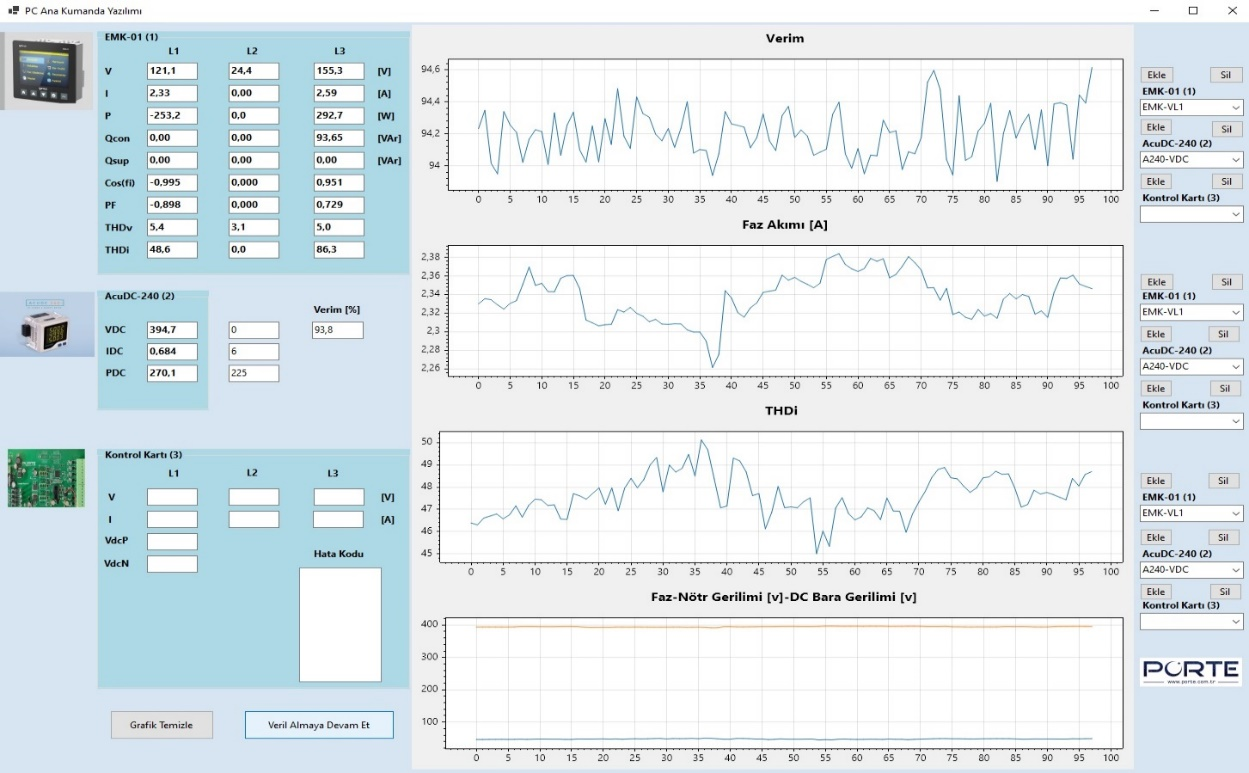
\includegraphics[width=0.98\textwidth]{deneysel/onceki_tez_sekil_5_19_susturma_pc.jpeg}
  \caption{Nötr anahtar susturma modunda PC yazılımında elde edilen grafikler.}
  \label{fig:deney-susturma-pc}
\end{figure}

Şekil~\ref{fig:deney-susturma-l1}, anahtarlamalı endüktör akımının sıfır çevresinde kesildiği aralıkları göstermektedir. Gözlenen zarf, Bölüm~\ref{chap:anahtarlama} içindeki Senaryo~2 kayıtları ve üçüncü harmonik mekanizmasıyla nitel olarak uyumludur.

\begin{figure}[htbp]
  \centering
  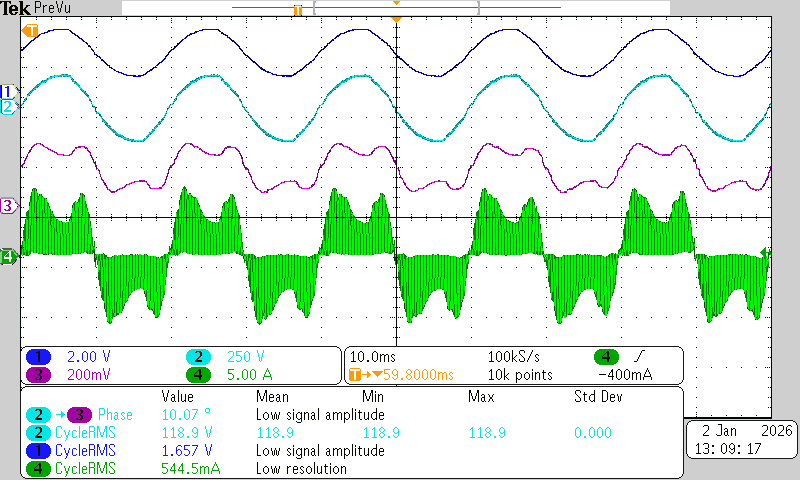
\includegraphics[width=0.94\textwidth]{deneysel/onceki_tez_sekil_5_20_susturma_l1.png}
  \caption{Susturma yönteminde kontrol işareti, şebeke gerilimi, ortalama endüktör akımı ve $L_1$ akımı.}
  \label{fig:deney-susturma-l1}
\end{figure}

Şekil~\ref{fig:deney-susturma-faz}, aynı yöntemin faz akımındaki belirgin biçim bozulmasını göstermektedir. Klasik yönteme göre farklı DA bara gerilimi kullanıldığından verim değişiminin tamamı yalnız anahtarlama yöntemine atfedilemez.

\begin{figure}[htbp]
  \centering
  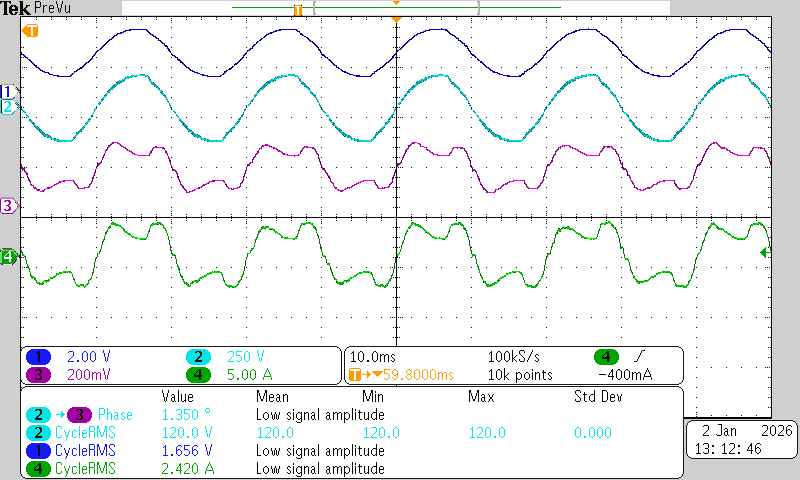
\includegraphics[width=0.94\textwidth]{deneysel/onceki_tez_sekil_5_21_susturma_faz.png}
  \caption{Susturma yönteminde kontrol işareti, şebeke gerilimi, ortalama endüktör akımı ve faz akımı.}
  \label{fig:deney-susturma-faz}
\end{figure}

\section{Susturma ve Sin\texorpdfstring{\textsuperscript{3}}{3} Modu Deney Kayıtları}

Üçüncü yöntemde nötr anahtar susturma korunmuş ve akım zarfındaki harmonik bozulmayı azaltmak amacıyla Sin\textsuperscript{3} tabanlı terim eklenmiştir. Deney özeti yüzde 94,5 verim, yüzde 14 akım THD'si, yaklaşık \SI{2.3}{\ampere} faz akımı, \SI{124}{\volt} faz--nötr gerilimi ve \SI{427}{\volt} DA bara gerilimi bildirmektedir. Benzetim modelinde terim $K_3\sin^3\theta$ biçimindedir (Bölüm~\ref{chap:sin3}); donanım yazılımı belgelenmediğinden deneydeki uygulamanın aynı biçimde olduğu kabul edilmiştir.

\begin{figure}[htbp]
  \centering
  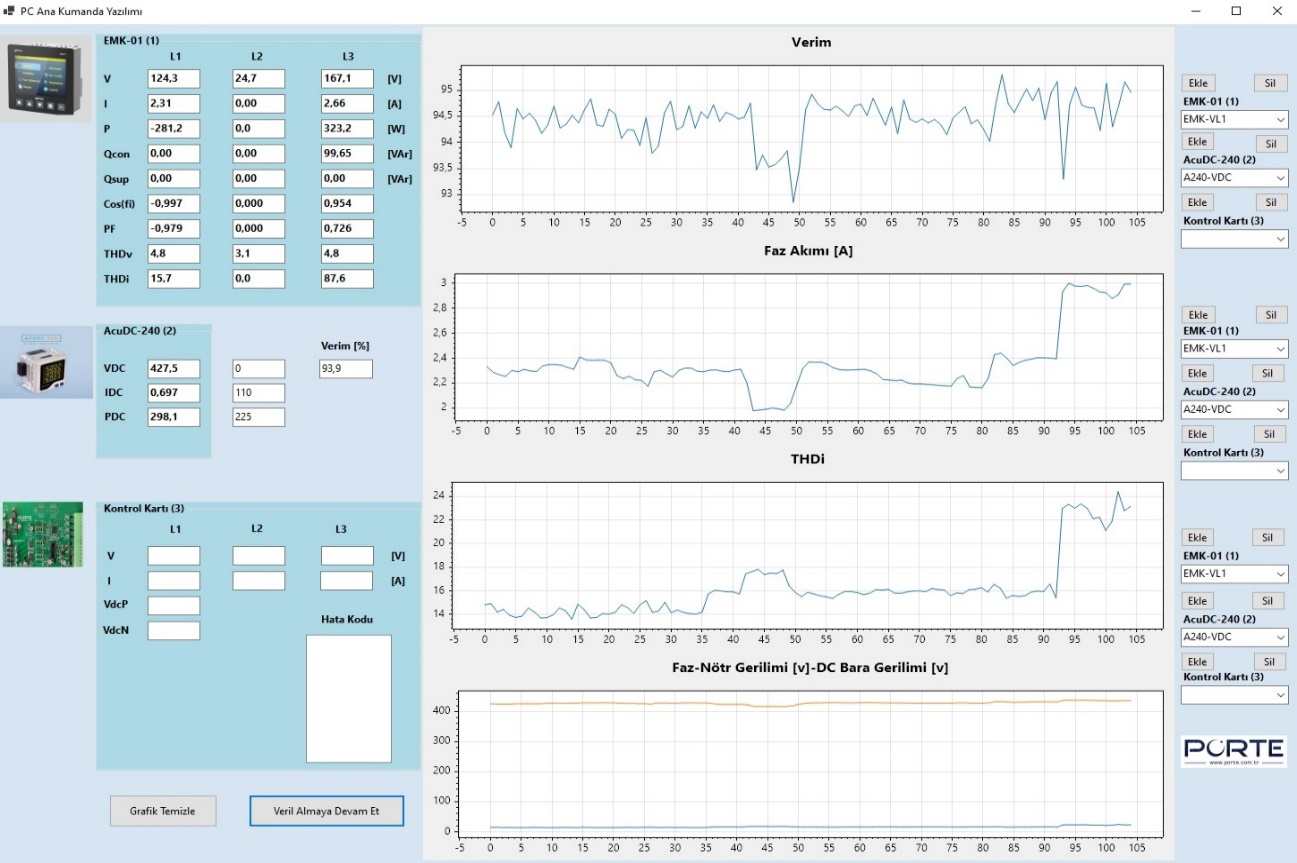
\includegraphics[width=0.98\textwidth]{deneysel/onceki_tez_sekil_5_22_sin3_pc.jpeg}
  \caption{Sin\textsuperscript{3} uygulanmış susturma modunda PC yazılımında alınan grafikler.}
  \label{fig:deney-sin3-pc}
\end{figure}

Şekil~\ref{fig:deney-sin3-l1}, susturma deneyine göre daha düzenli bir $L_1$ akım zarfı göstermektedir; nitel iyileşme, bildirilen THD azalmasıyla uyumludur.

\begin{figure}[htbp]
  \centering
  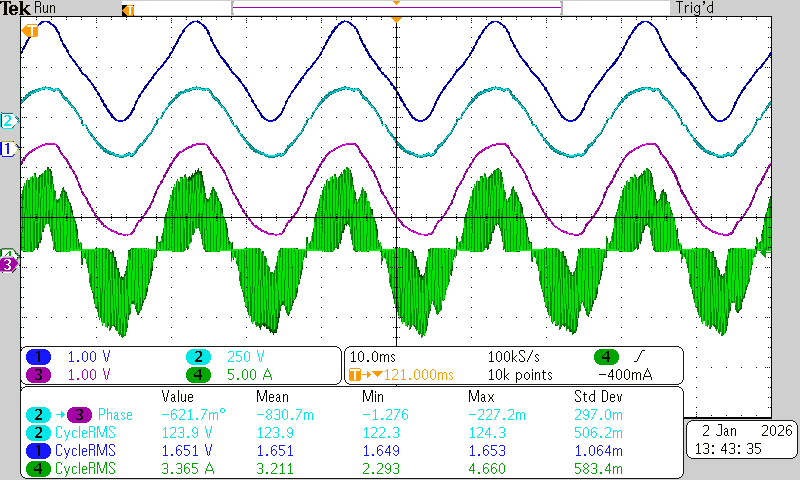
\includegraphics[width=0.94\textwidth]{deneysel/onceki_tez_sekil_5_23_sin3_l1.png}
  \caption{Sin\textsuperscript{3} uygulanmış yöntemde kontrol işareti, şebeke gerilimi, ortalama endüktör akımı ve $L_1$ akımı.}
  \label{fig:deney-sin3-l1}
\end{figure}

Şekil~\ref{fig:deney-sin3-faz}, faz akımındaki zarfın susturma yöntemine göre düzeldiğini göstermektedir. Klasik ve Sin\textsuperscript{3} deneyleri farklı DA bara ve faz gerilimlerinde yapıldığından tek değişkenli nedensel üstünlük sonucu çıkarılmamıştır.

\begin{figure}[htbp]
  \centering
  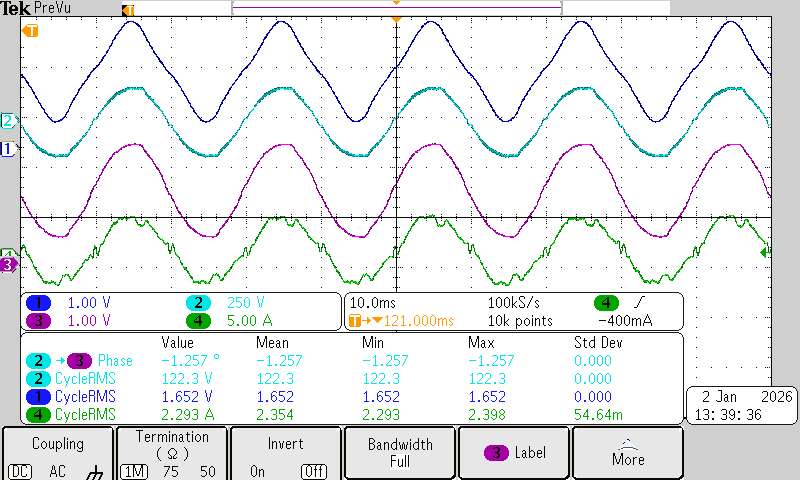
\includegraphics[width=0.94\textwidth]{deneysel/onceki_tez_sekil_5_24_sin3_faz.png}
  \caption{Sin\textsuperscript{3} uygulanmış yöntemde kontrol işareti, şebeke gerilimi, ortalama endüktör akımı ve faz akımı.}
  \label{fig:deney-sin3-faz}
\end{figure}

\section{Deney Sonuçlarının Değerlendirilmesi}

Üç yöntemin deneysel verim ve THD değerleri Tablo~\ref{tab:deney-dusuk-guc-ozeti} üzerindedir. Aynı noktalara kalibre edilen benzetim modelinin karşılık gelen değerleri, bağımsız doğrulama ölçütleriyle birlikte Kesim~\ref{sec:kalibrasyon} altında ayrı bir tabloda verilmektedir; benzetim ve deney değerleri aynı sütunda birleştirilmemiştir.

\begin{table}[htbp]
  \centering
  \caption{Üç yöntemin deneysel verim ve akım THD değerleri (deney özeti).}
  \label{tab:deney-dusuk-guc-ozeti}
  \footnotesize
  \begin{tabularx}{0.8\textwidth}{X >{\centering\arraybackslash}p{0.18\textwidth} >{\centering\arraybackslash}p{0.18\textwidth}}
    \toprule
    Yöntem & Verim & THD$_I$ \\
    \midrule
    Klasik tamamlayıcı anahtarlama & \%92,50 & \%15 \\
    Nötr anahtar susturma & \%94,20 & \%46 \\
    Susturma + Sin\textsuperscript{3} & \%94,50 & \%14 \\
    \bottomrule
  \end{tabularx}
\end{table}

Deney düzeneğindeki güç, ölçüm ve veri toplama akışı Şekil~\ref{fig:deney-olcum-zinciri} üzerinde özetlenmiştir.

\begin{figure}[htbp]
  \centering
  \begin{tikzpicture}[
    node distance=8mm and 10mm,
    block/.style={draw=blue!55!black,fill=blue!7,rounded corners,align=center,minimum height=10mm,text width=28mm,font=\small},
    meas/.style={draw=green!50!black,fill=green!8,rounded corners,align=center,minimum height=10mm,text width=28mm,font=\small},
    data/.style={draw=orange!70!black,fill=orange!10,rounded corners,align=center,minimum height=10mm,text width=30mm,font=\small},
    arr/.style={-{Latex[length=2.5mm]},thick}
  ]
    \node[block] (dc) {DA bara\\AcuDC240 + şönt};
    \node[block,right=of dc] (inv) {T-tipi evirici\\LCL filtre};
    \node[block,right=of inv] (grid) {Varyak ve\\AA şebeke};
    \draw[arr] (dc) -- node[above,font=\scriptsize] {$P_{dc}$} (inv);
    \draw[arr] (inv) -- node[above,font=\scriptsize] {$v_g,i_g$} (grid);
    \node[meas,below=of inv] (scope) {Osiloskop\\$i_{L1}$, $i_g$, $v_g$, DAC};
    \node[meas,below=of grid] (ac) {EMK-01 + CT\\$P_{ac}$, THD, PF};
    \node[meas,below=of dc] (ctrl) {Kontrol/ölçüm kartı\\ADC, PWM, FAULT};
    \draw[arr] (inv) -- (scope);
    \draw[arr] (grid) -- (ac);
    \draw[arr] (inv) -- (ctrl);
    \node[data,below=15mm of scope] (pc) {PC ana kumanda yazılımı\\RS485/Modbus RTU};
    \draw[arr] (ctrl) -- (pc);
    \draw[arr] (ac) -- (pc);
    \draw[arr] (dc) |- (pc);
    \draw[arr,dashed] (scope) -- node[right,font=\scriptsize] {ekran kaydı} (pc);
  \end{tikzpicture}
  \caption{Deney düzeneğindeki güç, ölçüm ve veri toplama akışı.}
  \label{fig:deney-olcum-zinciri}
\end{figure}

Tablo~\ref{tab:olcum-cihazlari}, kullanılan cihaz ve sensörleri doğrulama sınırlarıyla birlikte toplamaktadır. Kayıtlardaki ``Class 0,1'' ve AcuDC240 yüzde hata değerleri aynı büyüklük olarak kabul edilmemiş; osiloskop için yazılan ``300 Hz'' ifadesi model ailesiyle uyuşmadığından üretici belgesi bekleyen kayıt olarak işaretlenmiştir.

\begin{table}[htbp]
  \centering
  \caption{Ölçüm cihazları ve doğrulama sınırları.}
  \label{tab:olcum-cihazlari}
  \footnotesize
  \begin{tabularx}{\textwidth}{p{0.19\textwidth} p{0.23\textwidth} p{0.20\textwidth} X}
    \toprule
    Büyüklük & Cihaz / sensör & Bildirilen özellik & Doğrulama notu \\
    \midrule
    AA güç ve THD & Entes EMK-01 ve 50/5 oranlı, \SI{5}{\volt\ampere} akım transformatörleri & Class 0.1 & Kalibrasyon belgesi bağımsız olarak mevcut değildir. \\
    DA güç & Accuenergy AcuDC240 ve \SI{20}{\ampere}/\SI{60}{\milli\volt} şönt & Akım/gerilim yüzde 0,2; güç/enerji yüzde 0,5 & ``Class 0,1'' ifadesiyle uyuşmazlık üretici belgesiyle kesinleştirilecektir. \\
    Hızlı akım & Tektronix TCP0150 & \SI{150}{\ampere}, \SI{20}{\mega\hertz} & Prob oranı ham osiloskop dosyasıyla doğrulanacaktır. \\
    Hızlı gerilim & Tektronix THDP0200 & \SI{1500}{\volt}, \SI{200}{\mega\hertz} & Kanal zayıflatması ve ortak-mod sınırı ham kayıtla doğrulanacaktır. \\
    Osiloskop & Tektronix DPO3034 & Kayıtta ``300 Hz, 2,5 GS/s'' & ``300 Hz'' ifadesi model veri sayfasıyla uyuşmadığından bant genişliği doğrulanmalıdır. \\
    Faz/LCL akımı & HLSR 20-P/SP33 & \SI{23}{\milli\volt\per\ampere}; \SI{39.9}{\ampere} RMS hesap sınırı & Kazanç ve ADC ölçekleme katsayıları kontrol koduyla doğrulanacaktır. \\
    Gerilim ölçümü & AMC1200 tabanlı izole kart & Kazanç 8; \SI{2.6}{\volt} ADC aralığı & Direnç oranı ve kanal kalibrasyonu şemadan doğrulanacaktır. \\
    \bottomrule
  \end{tabularx}
\end{table}

Üç yöntemin çalışma koşulları Tablo~\ref{tab:deney-kosullari} üzerinde karşılaştırılmıştır. Yöntemler tam olarak aynı DA bara ve faz gerilimlerinde çalıştırılmadığından, verim sıralaması tek değişkenli bir yöntem karşılaştırması değildir.

\begin{table}[htbp]
  \centering
  \caption{Üç yöntem için bildirilen çalışma koşulları.}
  \label{tab:deney-kosullari}
  \footnotesize
  \begin{tabularx}{\textwidth}{p{0.21\textwidth} *{3}{>{\centering\arraybackslash}X} X}
    \toprule
    Büyüklük & Klasik & Nötr susturma & Susturma+Sin\textsuperscript{3} & Yorum \\
    \midrule
    Faz akımı & \SI{2.3}{\ampere} & \SI{2.3}{\ampere} & \SI{2.3}{\ampere} & Düşük güç noktası; anma testi değildir. \\
    Faz--nötr gerilimi & \SI{120}{\volt} & \SI{120}{\volt} & \SI{124}{\volt} & Yöntemler tam aynı gerilimde değildir. \\
    DA bara gerilimi & \SI{430}{\volt} & \SI{395}{\volt} & \SI{427}{\volt} & Yöntemler tam aynı bara koşulunda değildir. \\
    Analizörün $\cos\varphi$ göstergesi & $-0{,}990$--$1{,}000$ & $-0{,}995$ & $-0{,}997$ & Temel bileşen yer değiştirme faktörüdür; işaret kuralı belgelenmemiştir (Kesim~\ref{sec:kalibrasyon}). \\
    \bottomrule
  \end{tabularx}
\end{table}

Deney özet değerleri ile PC ekranlarında görünen anlık değerler de birebir aynı değildir; Tablo~\ref{tab:deney-metin-ekran-karsilastirma} farkları görünür kılmaktadır. Ekran değeri, görselde okunabilen tek anlık görüntüdür; özet değeri deney raporundaki sayıdır. Ham kayıtlar bulunmadan farkların ortalama, medyan, seçilmiş an veya farklı faz sonucu olup olmadığı belirlenemez; tablo bir hata düzeltme tablosu değil, kaynak içi tutarlılık denetimidir.

\begin{table}[htbp]
  \centering
  \caption{Deney özeti ile PC ekranlarında okunabilen anlık değerlerin karşılaştırılması.}
  \label{tab:deney-metin-ekran-karsilastirma}
  \footnotesize
  \begin{tabularx}{\textwidth}{p{0.21\textwidth} p{0.16\textwidth} >{\centering\arraybackslash}X >{\centering\arraybackslash}X X}
    \toprule
    Yöntem & Büyüklük & Özet & PC ekranı & Farkın durumu \\
    \midrule
    Klasik & Verim & \%92,5 & \%92,9 & Ortalama/anlık ayrımı doğrulanamadı. \\
    Klasik & THD$_i$ & \%15 & \%11,1 & Analiz penceresi ve ortalama yöntemi eksik. \\
    Klasik & $V_{dc}$ & \SI{430}{\volt} & \SI{431.5}{\volt} & Yakın değerler. \\
    \midrule
    Nötr susturma & Verim & \%94,2 & \%93,8 & Ortalama/anlık ayrımı doğrulanamadı. \\
    Nötr susturma & THD$_i$ & \%46 & \%48,6 & Aynı yüksek bozulma eğilimi; sayısal fark açık. \\
    Nötr susturma & $V_{dc}$ & \SI{395}{\volt} & \SI{394.7}{\volt} & Yakın değerler. \\
    \midrule
    Susturma+Sin\textsuperscript{3} & Verim & \%94,5 & \%93,9 & Ortalama/anlık ayrımı doğrulanamadı. \\
    Susturma+Sin\textsuperscript{3} & THD$_i$ & \%14 & \%15,7 & Aynı iyileşme eğilimi; sayısal fark açık. \\
    Susturma+Sin\textsuperscript{3} & $V_{dc}$ & \SI{427}{\volt} & \SI{427.5}{\volt} & Yakın değerler. \\
    \bottomrule
  \end{tabularx}
\end{table}

Deneysel kayıtlar yalnız yaklaşık \SI{2.3}{\ampere} düşük güç noktasını belgelemektedir. Orta ve anma akımında aynı denetim yapısının davranışı S4 benzetim taramasıyla (Kesim~\ref{sec:s4-kapali-cevrim}) incelenmiştir; Tablo~\ref{tab:deney-juri-durum}, güç bölgelerine göre deneysel ve benzetim kanıtını ayırmaktadır.

\begin{table}[htbp]
  \centering
  \caption{Doğrulamanın güç bölgelerine göre kanıt düzeyi.}
  \label{tab:deney-juri-durum}
  \small
  \begin{tabularx}{\textwidth}{p{0.17\textwidth} X X p{0.21\textwidth}}
    \toprule
    Çalışma bölgesi & Deneysel kanıt & Benzetim kanıtı & Tezdeki kullanım \\
    \midrule
    Düşük güç (\SI{2.3}{\ampere}) & Üç yönteme ait PC ve osiloskop ekranları; deney özeti & S1--S3 kalibre benzetimi (Tablo~\ref{tab:kalibrasyon-karsilastirma}); S4 \SI{2.3}{\ampere} koşuları & Destekleyici deneysel kanıt ve kalibre benzetim \\
    Orta güç (\SI{10}{\ampere}) & Kayıt yok & S4 P, PI, PIR koşuları (Tablo~\ref{tab:s4-tarama}) & Yalnız benzetim bulgusu \\
    Anma (\SI{25}{\ampere}) & Kayıt yok & S4 P, PI, PIR koşuları; büyütülmüş DA bara (Tablo~\ref{tab:s4-tarama}) & Yalnız benzetim bulgusu \\
    Geçici rejim & Kayıt yok & S4 \SI{10}{\ampere}$\rightarrow$\SI{25}{\ampere} basamağı (Tablo~\ref{tab:s4-basamak}) & Yalnız benzetim bulgusu \\
    \bottomrule
  \end{tabularx}
\end{table}

Orta ve anma gücünde deney yapılamamasının iki nedeni vardır. Birincisi, laboratuvar şebeke bağlantısının varyak üzerinden yaklaşık \SI{120}{\volt} ile sınırlı olmasıdır; anma gücü ifadeleri donanımın tasarım hedefi olarak kalmaktadır. İkincisi, deney donanımının DA bara kapasitörleri \SI{25}{\ampere} faz akımında bara orta noktasını tutamamaktadır (Kesim~\ref{sec:s4-kapali-cevrim}). Şebeke gerilimi ve DA bara sınırları nedeniyle orta ve anma akımı sonuçları deneyle doğrulanmamış benzetim bulgusu olarak raporlanmaktadır. Deneysel verimin belirsizliği için yalnız bir alt sınır verilebilir: DA analizörünün bildirilen yüzde 0,5 güç toleransı, birleşik belirsizliğin $u_{\eta}=\eta\sqrt{(u_{P_{ac}}/P_{ac})^2+(u_{P_{dc}}/P_{dc})^2}$ ilk yaklaşımında AA tarafı katkısı olmadan da \%94 verimde yaklaşık $\pm0{,}5$ puan verir. S2 ile S3 arasındaki 0,3 puanlık deneysel verim farkı belirsizlik alt sınırının içindedir.

\subsection{Deney Özet Tablosunun Sayısal Denetimi}

17.08.2026 tarihli çalışma kitabının gerçek uygulama alanı Senaryo~1--3 için tek satırlık özetler içermekte, ham zaman serisi veya tekrar koşusu vermemektedir. Tablo~\ref{tab:gelen-excel-senaryolar}, hücrelerdeki değerleri değiştirmeden ve $\eta_{VI}=100P_{\mathrm{out}}/(V_{\mathrm{dc}}I_{\mathrm{dc}})$ bağımsız hesabını ayrıca göstererek kaynağın izini korumaktadır.

\begin{table}[htbp]
  \centering
  \caption{Deney özet tablosundaki değerler ve DA giriş çarpımından yeniden hesaplanan verim.}
  \label{tab:gelen-excel-senaryolar}
  \footnotesize
  \begin{tabularx}{\textwidth}{c r r r r r r r}
    \toprule
    Senaryo & $V_{dc}$ (V) & $I_{dc}$ (A) & $V_{ac}$ (V RMS) & $I_{faz}$ (A) & $P_o$ (W) & THD (\%) & $\eta_{VI}$ (\%) \\
    \midrule
    1 & 431,5 & 0,624 & 119,8 & 2,26 & 249,6 & 15 & 92,700 \\
    2 & 395,0 & 0,684 & 121,0 & 2,33 & 253,2 & 47 & 93,715 \\
    3 & 427,5 & 0,697 & 124,3 & 2,31 & 281,2 & 14 & 94,373 \\
    \bottomrule
  \end{tabularx}
\end{table}

Bildirilen verimler sırasıyla \%92,5, \%94,2 ve \%94,5'tir; yeniden hesaplanan değerlerle farklar yaklaşık $-0{,}20$, $+0{,}48$ ve $+0{,}13$ yüzde puandır. Farkların yuvarlama, farklı ortalama penceresi veya ek kayıp teriminden kaynaklanıp kaynaklanmadığı ham güç örnekleri olmadan çözülemez. Kitabın benzetim satırları aynı temel sayıları tekrar etmekte, bağımsız Simulink çıktısı ya da ham iz sağlamamaktadır; tablo yalnız deneysel özet olarak kullanılmış, benzetim doğrulaması sayılmamıştır. Benzetim karşılaştırması, Kesim~\ref{sec:kalibrasyon} altında model koşularından yapılmıştır.

\section{Benzetim Modelinin Deney Özetine Kalibrasyonu}
\label{sec:kalibrasyon}

Deney özeti ile benzetim modelinin karşılaştırılabilmesi için S1--S3 benzetim modelleri deney özetinin çalışma noktalarına kalibre edilmiştir. Kesimin amacı, modelin deneyin hangi büyüklüklerini hangi hatayla yeniden ürettiğini göstermek ve kalibre benzetimi deney bulgusundan ayrı tutmaktır. Taban modeller, Kesim~\ref{sec:model-dogrulama-duzeltme} altında özetlenen düzeltmelerin uygulandığı S1, S2 ve S3 modelleridir. Kalibre değerler Tablo~\ref{tab:sistem-parametreleri} içinde ``Kalibre'' türüyle, parametre dosyasındaki ilk değerleri parantez içinde olmak üzere verilmiştir; S4 ileri beslemesi kalibre S3 değerlerini kullanır.

\subsection{Yöntem}

Devre, yarı iletken ve filtre parametreleri kalibrasyonda değiştirilmemiştir. Her senaryoda yalnız iki serbest değişken vardır: modülasyon genlik ölçeği ($K_{1x}$; S3'te $K_3/K_1$ oranı sabit tutularak $K_{13}$ ile $K_{33}$ birlikte) ve şebekeye göre referans fazı $\varphi_x$. İki serbest değişken iki hedefe ayarlanmıştır: etkin güç $P_{\mathrm{ac}}$ deney değerinin $\pm$\%1'i içinde, temel bileşen reaktif gücünün büyüklüğü $|Q_1|$ ise deneydeki $\cos\varphi$ okumasının yuvarlama bandı içinde tutulmuştur. AA çıkış akımı $I_{\mathrm{ac}}$, verim, DA güç ve akımı, $|\cos\varphi_1|$, güç faktörü ve akım THD'si kalibre edilmemiştir ve bağımsız doğrulama ölçütüdür. THD hedefi olarak deney özetinin \%15, \%47 ve \%14 değerleri alınmış, THD birincil ölçütler olan $P_{\mathrm{ac}}$, $I_{\mathrm{ac}}$ ve verimin ardından ikincil ölçüt olarak değerlendirilmiştir.

\textbf{Reaktif güç işareti ve ölçüm noktası.} Benzetimde güç büyüklükleri evirici çıkış uçlarında, yani EMC süzgecinden sonra ve $L_2$ ile temsil edilen şebeke ve varyak eşdeğerinden önce ölçülmektedir; nokta, deneyde AA analizörünün bağlı olduğu yaklaşık \SI{120}{\volt} tarafına karşılık gelir. İşaret kuralı üreticidir: evirici$\rightarrow$şebeke yönü pozitiftir, $Q_1>0$ akımın gerilimin gerisinde olduğu ve eviricinin şebekeye reaktif güç verdiği durumdur. Benzetimdeki pozitif $Q_1$'in kaynağı filtre kapasitörüdür. Deney özetindeki reaktif güç ölçülmemiş, $Q_o=P_o\tan(\arccos\cos\varphi)$ ile hesaplanmıştır ve eksi işareti analizörün $\cos\varphi$ göstergesinden gelir. Analizörün yön ve öncü/artçı kuralı belgelenmediğinden işaret yorumlanmamış, karşılaştırma büyüklükler ($|Q_1|$, $|\cos\varphi_1|$) üzerinden yapılmıştır. Deneydeki $\cos\varphi$, temel bileşen yer değiştirme faktörüdür ($\cos\varphi_1$) ve toplam güç faktöründen ($\mathrm{PF}=P/(V_{\mathrm{rms}}I_{\mathrm{rms}})$) ayrı raporlanmıştır. Üç basamaklı $\cos\varphi$ okuması $|Q_1|$ için S1'de 0--7,9~var, S2'de 24,1--26,7~var, S3'te 19,9--23,6~var bandı verir; şebeke gerilimi okumasının \SI{0.1}{\volt} çözünürlüğü $|Q_1|$'de yaklaşık $\pm12$~var belirsizlik doğurduğundan $|Q_1|$ uyumsuzluğu tek başına modeli reddettirmez. Deney iki işaret dalını ayırt edemediğinden her senaryoda kalibrasyonsuz modelin dalı ($Q_1>0$) korunmuştur.

\textbf{Köprünün yumuşak kaynak davranışı.} İlk kalibrasyon adımları, evirici köprüsünün temel bileşen geriliminin modülasyonla bire bir kaymadığını göstermiştir. Köprü, koşulardan ölçülen bir Thevenin eşdeğeriyle temsil edildiğinde iç empedansın büyüklüğü S1'de \SI{1.67}{\ohm}, S2'de \SI{28.7}{\ohm}, S3'te \SI{13.7}{\ohm} çıkmıştır. S1'deki değer, tamamlayıcı anahtarlamada akım dalgalanmasının her periyotta sıfırı kesmesiyle \SI{1}{\micro\second} ölü zamanın akıma bağlı gerilim hatası üretmesinden kaynaklanır; kaba ölü zaman kestirimi de yaklaşık \SI{1.7}{\ohm} verir. S2 ve S3'te köprü, son \SI{20}{\milli\second}'lik pencerenin \%12,4 ve \%22,6'sında süreksiz iletimdedir; susturmalı köprü düşük akımda akım kaynağına yaklaşır ve senkron olmayan buck eşdeğeriyle aynı davranışı gösterir (Kesim~\ref{sec:dusuk-akim-modelleme}). Thevenin empedansı LCL ağının \SI{50}{\hertz} empedansından büyük olduğundan etkin güç esas olarak genlikle, reaktif güç esas olarak fazla değişmektedir. İki değişken birbirini etkilediği için hedefler, koşulardan öğrenilen ampirik Jacobian ile iki boyutlu Newton yinelemesiyle birlikte çözülmüştür; S1 ve S2'de dört, S3'te altı kalibrasyon koşusu gerekmiştir.

\subsection{Kalibrasyon sonucu ve bağımsız karşılaştırma}

Kalibrasyon S1'de genliği değiştirmemiş (\%0,0003), fazı $+0{,}074^{\circ}$ kaydırmıştır; parametre dosyasındaki genlik deneyin etkin gücünü \%0,96 içinde zaten vermektedir ve faz düzeltmesi yalnız $|Q_1|$'i bant içine taşır. S2'de genlik \%3,3, S3'te \%1,5 azalmış, fazlar $+0{,}11^{\circ}$ ve $+0{,}66^{\circ}$ kaymıştır. Genlik belirsizliği deney toleransının ölçülen duyarlılıklara bölünmesiyle S1'de $\pm$\%0,025, S2'de $\pm$\%0,4, S3'te $\pm$\%0,2; faz belirsizliği sırasıyla $\pm0{,}05^{\circ}$, $\pm0{,}4^{\circ}$ ve $\pm0{,}5$--$1^{\circ}$ bulunmuştur. S2 ve S3 fazları faz belirsizliğinin içindedir ve fiziksel bir gecikme olarak yorumlanmamıştır. S2 ve S3'teki genlik azalması, yaklaşık \SI{50}{\micro\second}'lik ortalama iletim süresinde darbe başına 0,7--\SI{1.6}{\micro\second} kısalmaya eşdeğerdir; değer, modelde bulunmayan sürücü ve anahtar gecikmelerinin darbe genişliğinden yediği süre düzeyindedir. Yorum bir varsayımdır ve donanım kaydıyla doğrulanmamıştır.

\begin{table}[htbp]
  \centering
  \caption{Deney özeti ile kalibre benzetim modelinin karşılaştırılması. İlk iki satır kalibrasyon hedefidir; diğer satırlar kalibre edilmemiştir ve bağımsız karşılaştırmadır. Fark: \% göreli, ``p'' yüzde puan.}
  \label{tab:kalibrasyon-karsilastirma}
  \scriptsize
  \setlength{\tabcolsep}{2.6pt}
  \begin{tabular}{@{}l ccc ccc ccc@{}}
    \toprule
    & \multicolumn{3}{c}{S1 Klasik} & \multicolumn{3}{c}{S2 Susturma} & \multicolumn{3}{c}{S3 Susturma + Sin\textsuperscript{3}} \\
    \cmidrule(lr){2-4}\cmidrule(lr){5-7}\cmidrule(lr){8-10}
    Büyüklük & Deney & Benzetim & Fark & Deney & Benzetim & Fark & Deney & Benzetim & Fark \\
    \midrule
    $P_{\mathrm{ac}}$ (W) & 249,6 & 247,21 & $-$\%0,96 & 253,2 & 253,80 & $+$\%0,24 & 281,2 & 279,90 & $-$\%0,46 \\
    $|Q_1|$ (var) & 0--7,9 & 1,93 & bantta & 24,1--26,7 & 24,43 & bantta & 19,9--23,6 & 21,41 & bantta \\
    \midrule
    $I_{\mathrm{ac}}$ (A) & 2,26 & 2,218 & $-$\%1,8 & 2,33 & 2,416 & $+$\%3,7 & 2,31 & 2,279 & $-$\%1,4 \\
    $\eta$ (\%) & 92,5 & 91,15 & $-$1,35 p & 94,2 & 93,93 & $-$0,27 p & 94,5 & 94,25 & $-$0,25 p \\
    $P_{\mathrm{dc}}$ (W) & 269,26 & 271,21 & $+$\%0,7 & 270,18 & 270,19 & $+$\%0,004 & 297,97 & 296,97 & $-$\%0,34 \\
    $I_{\mathrm{dc}}$ (A) & 0,624 & 0,6286 & $+$\%0,7 & 0,684 & 0,6841 & $+$\%0,02 & 0,697 & 0,6947 & $-$\%0,32 \\
    THD$_I$ (\%) & 15 & 39,5 & $+$24,5 p & 47 & 56,7 & $+$9,7 p & 14 & 14,8 & $+$0,8 p \\
    $|\cos\varphi_1|$ & 1,000 & 0,99997 & $\approx0$ & 0,995 & 0,99538 & $+$0,0004 & 0,997 & 0,99708 & $+$0,0001 \\
    PF & 0,922 & 0,929 & $+$\%0,8 & 0,898 & 0,867 & $-$\%3,4 & 0,979 & 0,987 & $+$\%0,8 \\
    \bottomrule
  \end{tabular}
\end{table}

Tablo~\ref{tab:kalibrasyon-karsilastirma}, kalibre benzetimin deney özetiyle karşılaştırmasını vermektedir. Etkin güç ve reaktif güç büyüklüğü iki serbest değişkenle ayarlandığından ilk iki satırdaki uyum bir doğrulama değildir; doğrulama yalnız kalibre edilmeyen satırlardadır.

\textbf{S3.} Kalibre model deneyin AA akımını $-$\%1,4, verimini $-0{,}25$ puan, akım THD'sini $+0{,}8$ puan ve DA gücünü $-$\%0,3 hatayla yeniden üretmektedir. THD kalibre edilmemiştir: kalibrasyon öncesinde \%10,9 olan değer kalibrasyon sonrasında \%14,8 olmuştur (deney \%14). Sonuç, susturmalı çalışmanın düşük akımdaki dalga biçimi bozulmasının modelde doğru büyüklükte olduğunu gösteren en güçlü bağımsız kanıttır.

\textbf{S2.} Kalibre model DA gücünü ve DA akımını \%0,02 içinde, verimi $-0{,}27$ puan hatayla yeniden üretmektedir. AA akımı ise $+$\%3,7, THD $+9{,}7$ puan yüksektir; güç faktöründeki $-$\%3,4 fark aynı farkın sonucudur. Model S2'de deneyden daha bozuk bir akım vermektedir. İki serbest değişken etkin ve reaktif güce ayrıldığından fark kalibrasyonla kapanmaz. Olası kaynaklar, sıfır geçişi çevresindeki süreksiz iletim ayrıntısını belirleyen ve modelde bulunmayan IGBT çıkış kapasitesi ile sürücü gecikmeleri ve diyot toparlanma parametreleridir; kaynak ayrıştırılmamıştır.

\textbf{S1.} Kalibre model AA akımını $-$\%1,8, verimi $-1{,}35$ puan, DA gücünü $+$\%0,7 hatayla yeniden üretmektedir. Verim farkı, modelde \SI{24.0}{\watt}, deneyde \SI{19.7}{\watt} kayba karşılık gelir ve S1 için kayıp ayrıştırması yapılmamıştır. THD farkı ($+24{,}5$ puan) deney satırının iç tutarsızlığıyla birlikte okunmalıdır: deneyin $P/(VI)=0{,}922$ değeri $\cos\varphi_1=1$ ile ancak yaklaşık \%42 THD ile tutarlıdır; \%15 THD ile güç faktörü 0,989 olurdu. Modelin güç faktörü (0,929) deneyle \%0,8 içinde, THD'si \%39,5'tir. Model, deney satırındaki güç, gerilim ve akımla tutarlıdır; \%15 THD girdisiyle tutarlı değildir.

\textbf{Senaryo sıralaması.} Verim sıralaması S1 $<$ S2 $<$ S3, modelde ve deneyde aynıdır. S1$\rightarrow$S3 verim artışı modelde $+3{,}10$, deneyde $+2{,}0$ puan; S1$\rightarrow$S2 artışı modelde $+2{,}78$, deneyde $+1{,}7$ puandır. Fark esas olarak S1 verimindeki $-1{,}35$ puanlık sapmadan gelmektedir.

\textbf{Belirsizlik ve sınırlar.} Kararlı durum değerleri \SI{0.1}{\second} benzetimin son şebeke periyodundan alınmıştır. S2 ve S3'te son periyot ile 0,08--\SI{0.10}{\second} ortalaması arasında DA güçte 0,4--\SI{0.5}{\watt}, verimde 0,1 puana varan fark vardır; fark, verim karşılaştırmasının benzetim tarafı belirsizliğidir. Kalibre benzetim sonuçları deney bulgusu değildir; ``model, deneyin büyüklüğünü belirtilen hatayla yeniden üretmektedir'' biçiminde okunmalıdır. S2'nin AA akımı ve THD farkı, S1 deney satırının THD tutarsızlığı ve S1 verim farkı Bölüm~\ref{chap:sonuc} içinde sınırlılık olarak yer almaktadır.

\section{Bölüm Sonucu}

Deney düzeneği; T-tipi güç katı, faz modülleri, kontrol, tampon ve sürücü kartları, gerilim ve akım ölçüm devreleri, koruma devresi, AA ve DA analizörleri, şönt bağlantısı, PC yazılımı ve üç yönteme ait ekran kayıtlarıyla belgelenmiştir. Deney protokolü, ham kayıtlar ve tekrarlar mevcut olmadığından deney sonuçları ekran ve özet tablosu düzeyinde destekleyici kanıttır.

Üç yönteme ait kayıtlar, nötr susturmanın düşük güçte verimi artırırken harmonik bozulmayı büyüttüğü, Sin\textsuperscript{3} teriminin ise susturma kaynaklı bozulmayı azalttığı mekanizmasını nitel olarak desteklemektedir. Etkin ve reaktif güce kalibre edilen benzetim modeli, S3'te deneyin AA akımını \%1,4, verimini 0,25 puan ve kalibre edilmemiş akım THD'sini 0,8 puan içinde yeniden üretmekte ve deneyin verim sıralamasını korumaktadır; S2'de akım bozulmasını fazla, S1'de verimi düşük vermektedir. Özet ile ekran değerleri arasındaki farklar, yöntemler arasındaki DA bara ve şebeke gerilimi değişimi ve analizörün işaret kuralının belgelenmemesi açıkça gösterilmiştir. Orta ve anma akımı yalnız S4 benzetimiyle incelenmiştir; ortak koşullu ve anma gücünde deney yapılmamıştır.
